\documentclass{beamer}
\usepackage{beamerthemeshadow}
\usepackage{verbatim}

\usepackage{lastpage}
\usepackage{xcolor}
\usepackage{pgf}
\usepackage{colortbl}
\usepackage{hyperref}
\usepackage{multirow}
\usepackage{dsfont}
\usepackage{graphbox}

\newenvironment{benumerate}[1]{
  \let\oldItem\item
  \def\item{\addtocounter{enumi}{-2}\oldItem}
  \begin{enumerate}
    \setcounter{enumi}{#1}
    \addtocounter{enumi}{1}
}{\end{enumerate}}
                 

\usepackage{siunitx}
\sisetup{input-symbols=(), group-digits  = false} 

\newcommand{\bi}{\begin{itemize}}
\newcommand{\ei}{\end{itemize}}
\newcommand{\be}{\begin{enumerate}}
\newcommand{\ee}{\end{enumerate}}
\newcommand{\bd}{\begin{description}}
\newcommand{\ed}{\end{description}}
\newcommand{\prbf}[1]{\textbf{#1}}
\newcommand{\prit}[1]{\textit{#1}}
\newcommand{\beq}{\begin{equation}}
\newcommand{\eeq}{\end{equation}}
\newcommand{\bdm}{\begin{displaymath}}
\newcommand{\edm}{\end{displaymath}}

\newcommand{\ft}[1]{
  \frametitle{\begin{tabular}{p{4.2in}r} \textcolor{white}{#1} & \small{\insertframenumber / \inserttotalframenumber} \end{tabular}}
  \setbeamercovered{transparent=18}
}

\newcommand{\eft}[1]{
  \frametitle{\begin{tabular}{p{4in}r} \textcolor{white}{#1} & \small{\hyperlink{f:questions}{\beamergotobutton{GO BACK}}} \end{tabular}}
  \setbeamercovered{transparent=18}
}

\newcommand{\stepinv}{\setbeamercovered{invisible}}
\newcommand{\stopinv}{\setbeamercovered{transparent=18}}
\newcommand{\uncoverinv}[1]
{
  \setbeamercovered{invisible}
  \uncover<+->{#1}
  \setbeamercovered{transparent=18}
}
\newcommand{\ans}[1]{\textcolor{blue}{#1}}
\newcommand{\ansinv}[1]
{
  \setbeamercovered{invisible}
  \uncover<+->{\textcolor{blue}{#1}}
  \setbeamercovered{transparent=18}
}
\newcommand{\setinv}{\setbeamercovered{invisible}}
\newcommand{\setvis}{\setbeamercovered{transparent=18}}
\newcommand{\centerpic}[2]
{
  \begin{center}
  \includegraphics[#1]{#2}
  \end{center}
}
\newcommand{\h}[1]{\hat{#1}}
\newcommand{\ds}{\displaystyle}

\definecolor{light}{rgb}{1.0,0.7,0.7}
\definecolor{BrickRed}{rgb}{0.8,0.1,0.1}
%\definecolor{light}{rgb}{1.0,0.5,0.5}
%\newcommand{\hl}[1]{\only<#1>{\cellcolor{BrickRed}}}
\newcommand{\hl}[1]{\textcolor<#1>{BrickRed}}

\definecolor{mycolor}{rgb}{0.6,0.0,0.0}
\usecolortheme[named=mycolor]{structure}

\title[Predictors for Students' Understanding of Writing]{Predictors for Students' Understanding of Writing: Instructor Actions and Student Mindset}
\author[James M. Murray, University of Wisconsin - La Crosse]{
  \vspace*{-0.3in}\texorpdfstring{
    \small{
      \begin{columns}[t]
        \column{0.48\textwidth}
        \begin{center}
          Sara L. Cook\\
          Viterbo University\\
          \ \\
          Brenda L. Murray\\
          University of Wisconsin - La Crosse  
        \end{center}
        \column{0.48\textwidth}
        \begin{center}
          Sloan Komissarov\\
          Western Technical College\\
          \ \\
          \textcolor{mycolor}{James M. Murray\\
            University of Wisconsin - La Crosse\\
          (Presenter)}
        \end{center}
      \end{columns}
    }
  }{}
}

\date{
  \small{
    August 4, 2018\\
  \ \\
  Midwest Economics Research Group (MERG)\\
  2018 Annual Meeting
  }
}
\begin{document}

\frame{\titlepage \setcounter{framenumber}{0}}

\frame{
  \ft{Writing Purposes}
  \uncover<+->{
  \begin{block}{Demonstrate Understanding}
    \bi
    \item Exams
    \item Summarize concepts
    \item Connect ideas
    \ei
  \end{block}
  }

  \uncover<+->{
  \begin{block}{Personal Growth}
    \bi
    \item Write to learn
    \item Improve communication skills
    \item Genre-specific practice (business reports, lab reports, academic discourse)
    \ei
  \end{block}
  }

  \uncover<+->{
  \begin{block}{Audience-Driven Purpose}
    \bi
    \item Argue / Persuade
    \item Inform of research findings
    \item Inform decisions
    \ei
  \end{block}
  }
}

\frame{
  \ft{Writing Audience}
  \uncover<+-> {
  \begin{block}{The Instructor}
    \bi
    \item Ugh.. I'm not doing this for me.
    \item Appropriate for \textit{demonstrating understanding}
    \ei
  \end{block}
  }

  \uncover<+->{
  \begin{block}{Experts in Field or Similar}
    \bi
    \item Experts: Academic discourse
    \item Fellow students: Inform of research findings
    \item People with similar interests
    \ei
  \end{block}
  }

  \uncover<+->{
  \begin{block}{Authentic Audience}
    \bi
    \item Tied to purpose: Eg - persuade referendum voters 
    \item Fictional \& authentic tied to topic:\\
      Eg - board of directors, K-12 teachers, mental health care providers
    \ei
  \end{block}
  }
}

\frame{
  \ft{College Experience: Purpose \& Audience}

  \begin{columns}
  \uncover<+->{
    \begin{column}{0.50\textwidth}
      \begin{block}{Purposes (Previous Slide)}
        \be
        \item Demonstrate Understanding
        \item Personal Growth
        \item Audience-Driven
        \ee
      \end{block}
    \end{column}
  }
  \uncover<+->{
    \begin{column}{0.40\textwidth}
      \begin{block}{Audiences (Previous Slide)}
        \be
        \item Instructor
        \item Experts in Field
        \item Authentic
        \ee
      \end{block}
    \end{column}
  }
  \end{columns}

  \uncover<+->{
  \begin{block}{\textbf{Our Purpose \#1:} Measure College Student Experiences}
    \bi
    \item Place and purpose for all the above
    \item Measure students' perceptions
    \item Measure coverage of all the above
    \ei
  \end{block}
  }

  \uncover<+->{
  \begin{block}{\textbf{Our Purpose \#2:} Explore Determinants for Purposeful Writing}
    \bi
    \item Student mindset 
    \item Instructor actions
    \item Student background \& demographics
    \item Academic differences: field-of-study, year-in-school
    \ei
  \end{block}
  }
}


\frame
{
  \ft{Measuring Purpose}
  \uncover<+->{
  \begin{block}{Open-Ended Survey Question}
    Think about the last 3+ page writing assignment you completed. In one sentence \textbf{describe the purpose} for the writing
  \end{block}
  }
  \uncover<+->{  
  \begin{block}{Categorized Responses Into Ordered Levels} 
      \be
      \item None / unclear
      \item Topic or assignment description, instructor-centered
      \item Writer-centered (personal growth, practice)
      \item Reader-centered
        \ee
  \end{block}
  }
  \uncover<+->{  
  \begin{block}{Student Confidence in Answer}
    \vspace*{-1pc}\begin{columns}[t]
      \column{0.45\textwidth}
      \begin{benumerate}{4}
        \item Highly Confident
        \item Somewhat Confident
      \end{benumerate}

      \column{0.45\textwidth}
      \begin{benumerate}{2}
        \item Somewhat Not Confident 
        \item Not at all Confident
      \end{benumerate}
          
    \end{columns}
  \end{block}
  }
}

\frame
{
  \ft{Measuring Purpose}
  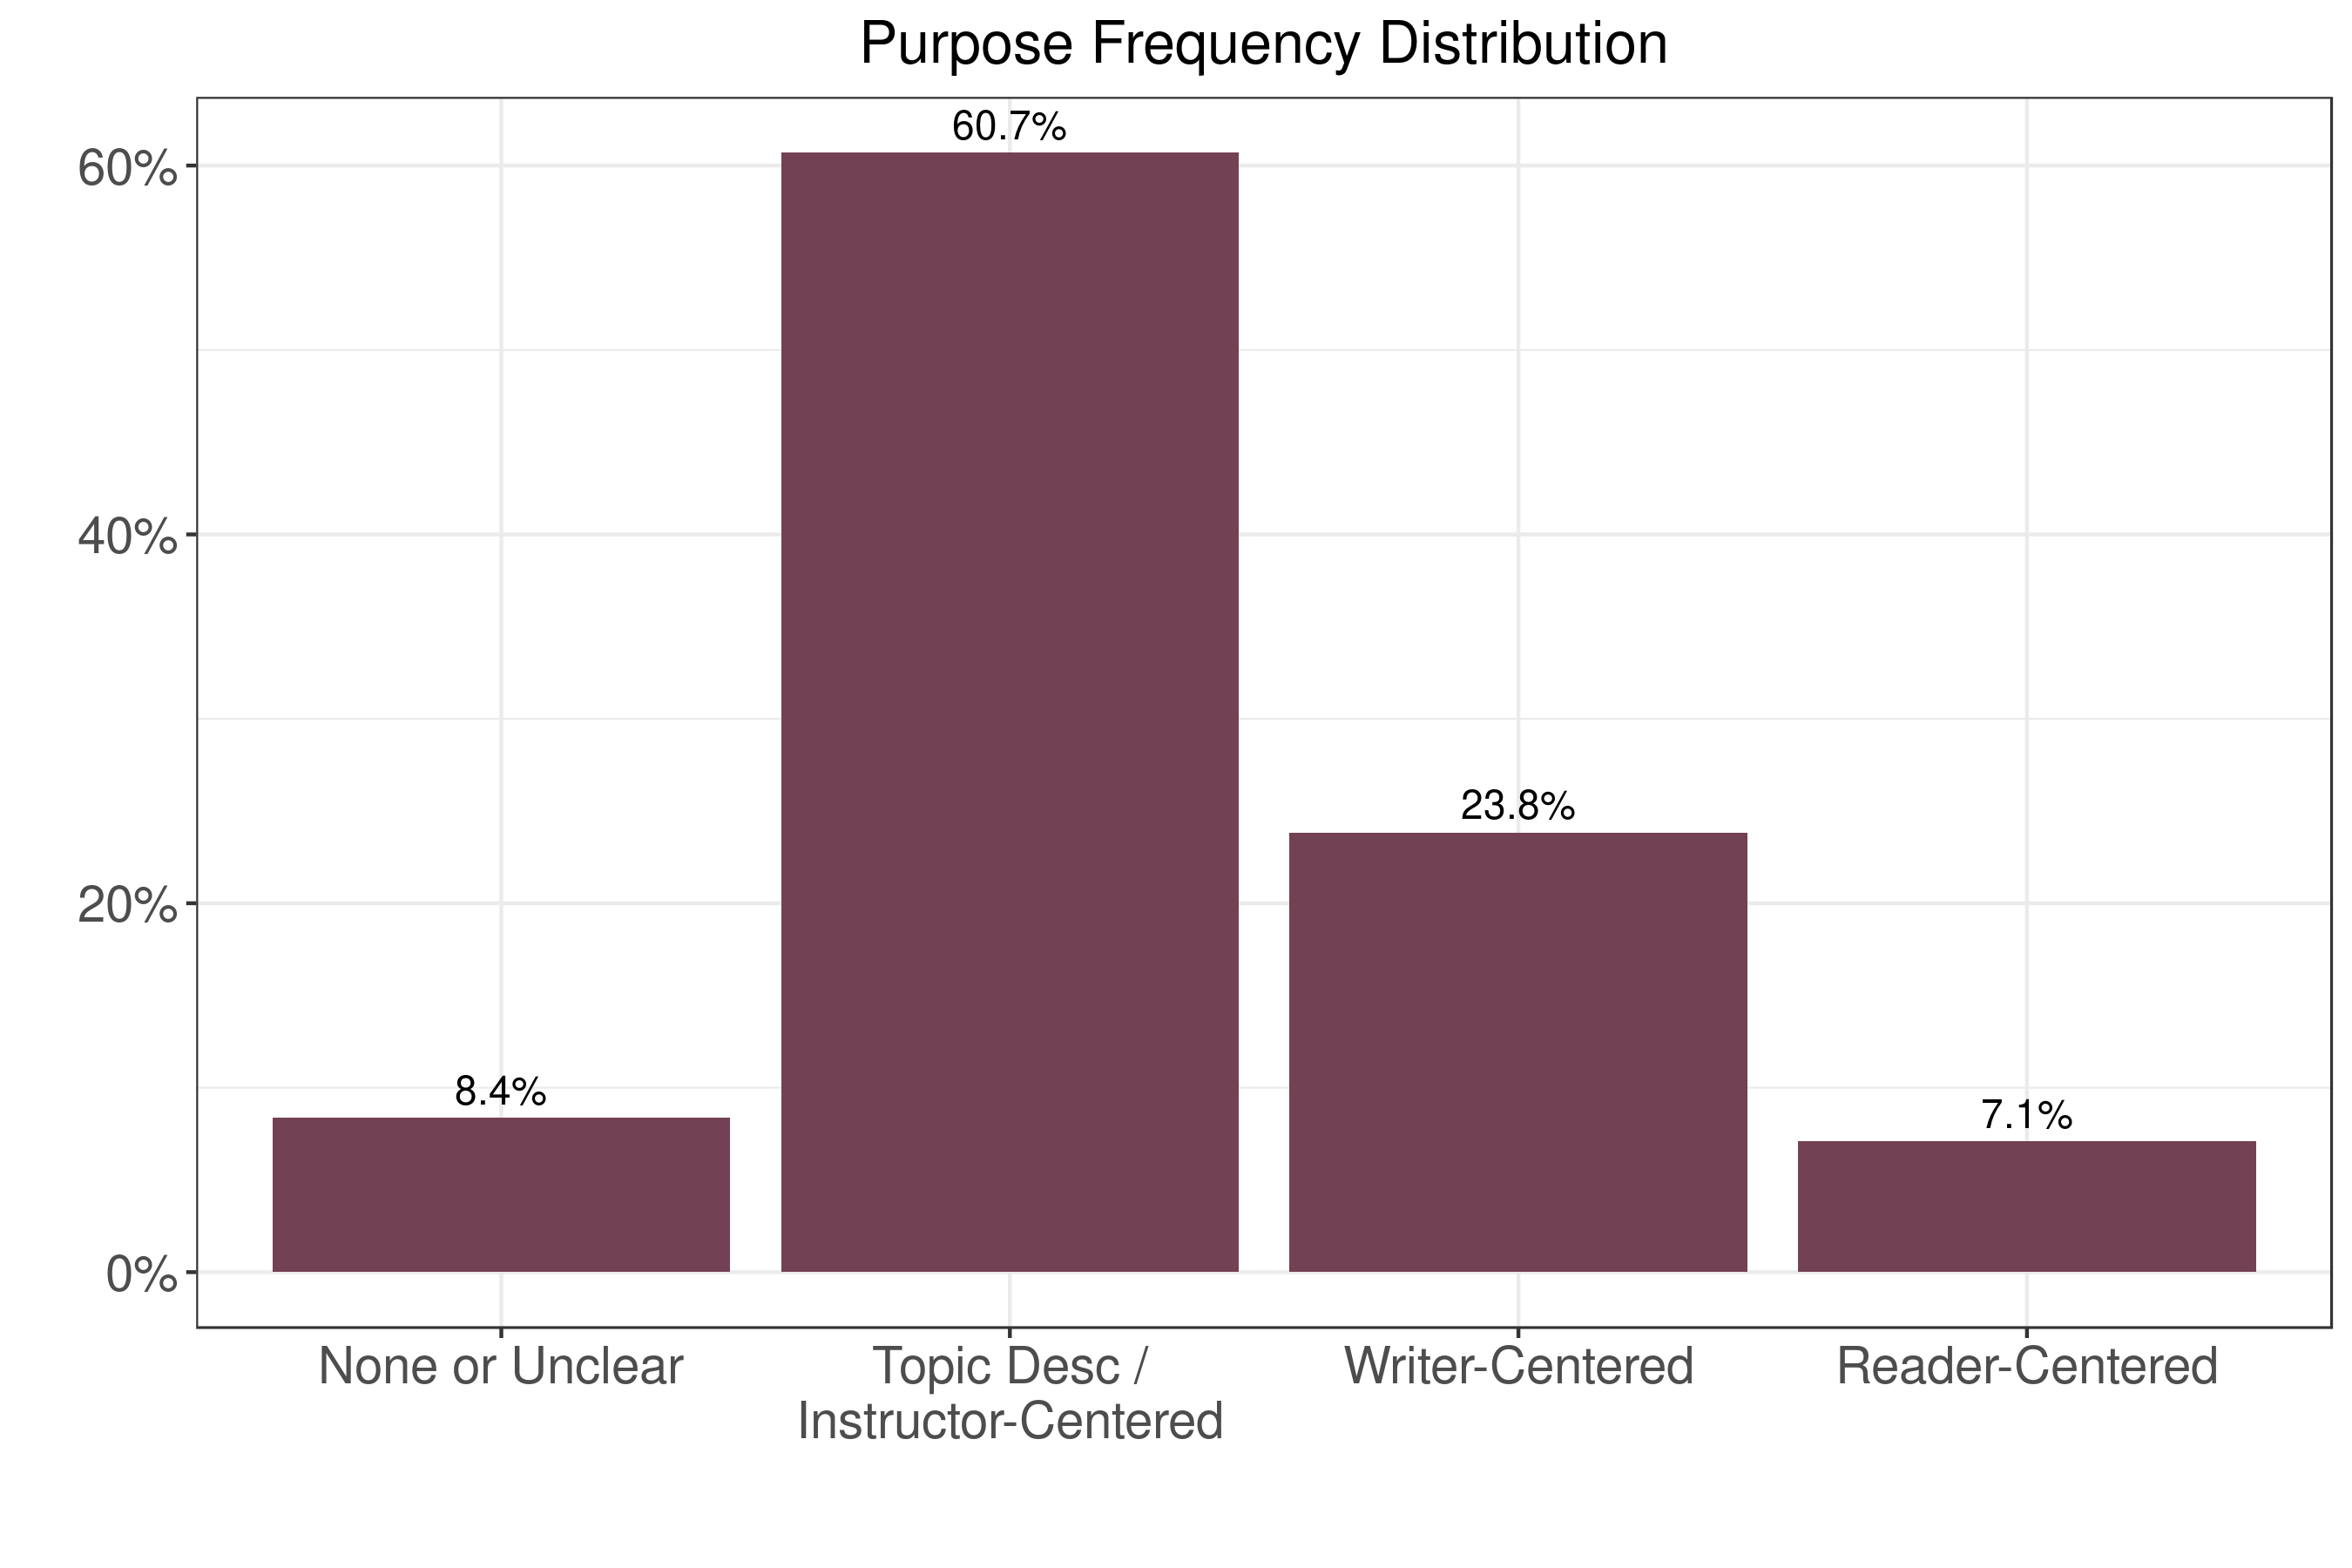
\includegraphics[width=\textwidth]{purpose-freq.png}
}

\frame
{
  \ft{Measuring Purpose}
  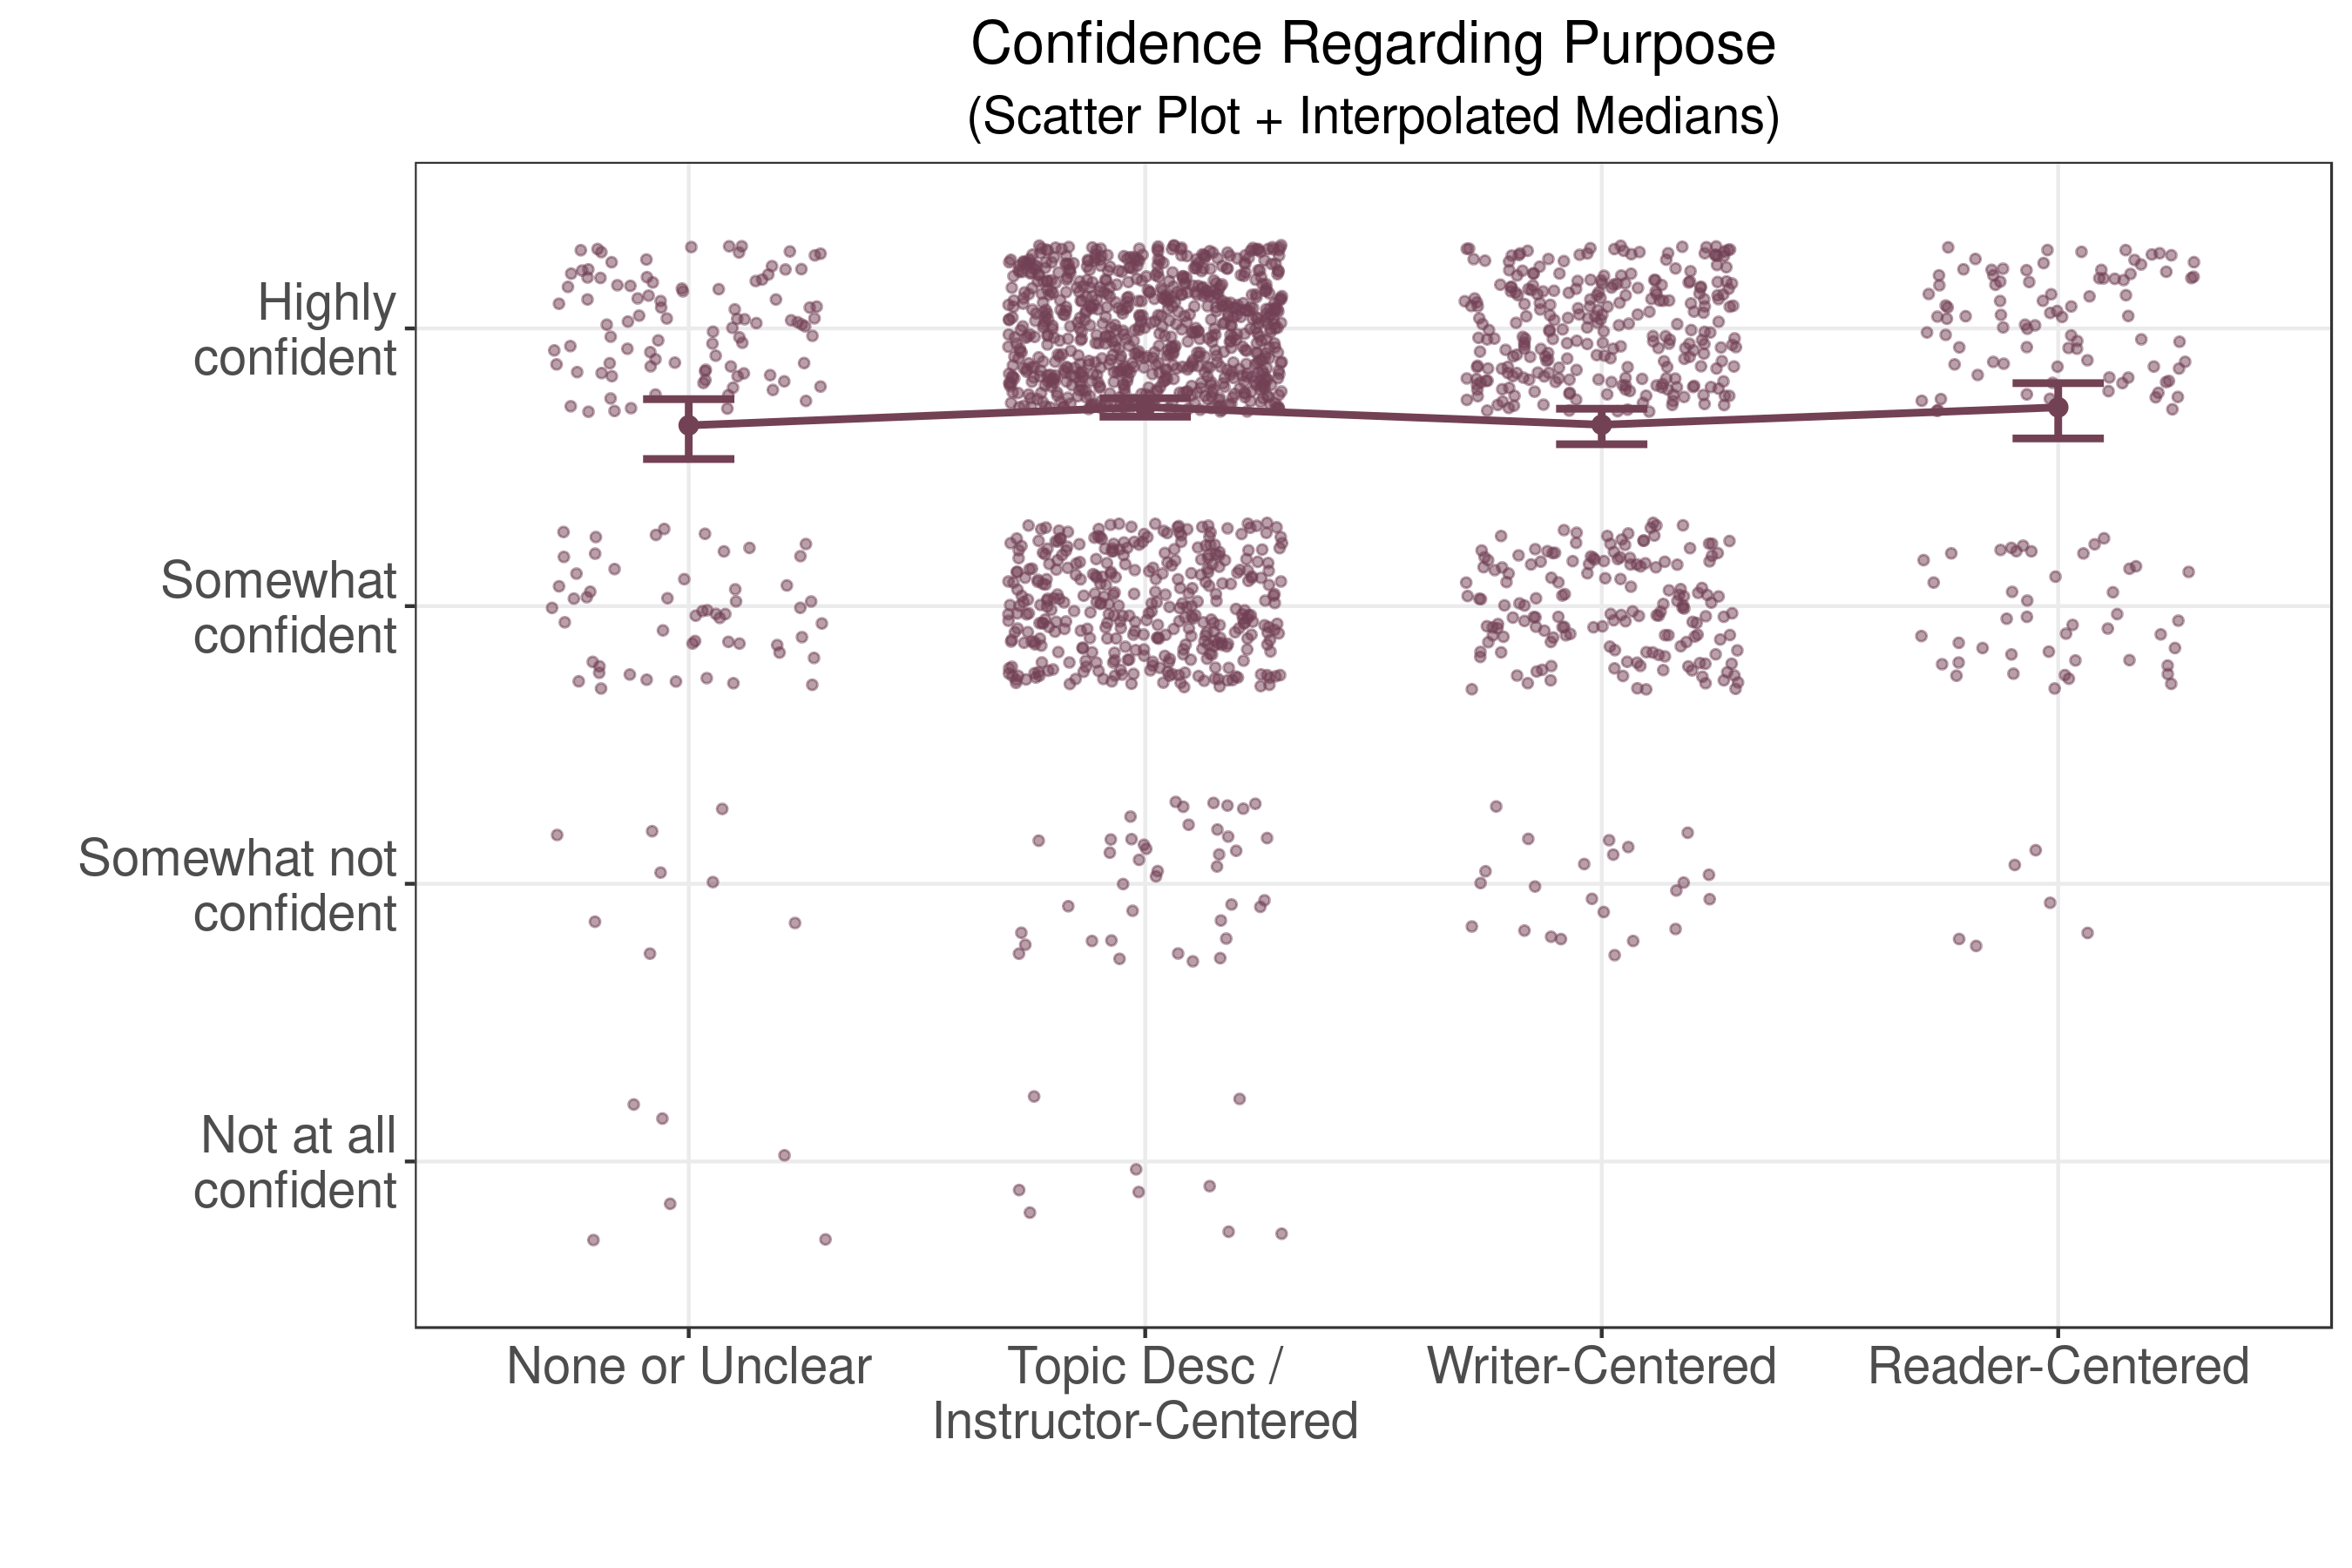
\includegraphics[width=\textwidth]{purpose-scat.png}
}


\frame
{
  \ft{Measuring Audience}
  \uncover<+->{  
  \begin{block}{Open-Ended Survey Question}
    Think about the last 3+ page writing assignment you completed. In one sentence \textbf{describe the audience} for the writing
  \end{block}
  }
  \uncover<+->{  
  \begin{block}{Categorized Responses Into Ordered Levels} 
      \be
      \item None / unclear
      \item Instructor-centered
      \item Subject matter experts, class peers, ``people interested in...'' 
      \item Authentic description
        \ee
  \end{block}
  }

  \uncover<+->{  
  \begin{block}{Student Confidence in Answer}
    \vspace*{-1pc}\begin{columns}[t]
      \column{0.45\textwidth}
      \begin{benumerate}{4}
        \item Highly Confident
        \item Somewhat Confident
      \end{benumerate}

      \column{0.45\textwidth}
      \begin{benumerate}{2}
        \item Somewhat Not Confident 
        \item Not at all Confident
      \end{benumerate}
          
    \end{columns}
  \end{block}
  }
}

\frame
{
  \ft{Measuring Audience}
  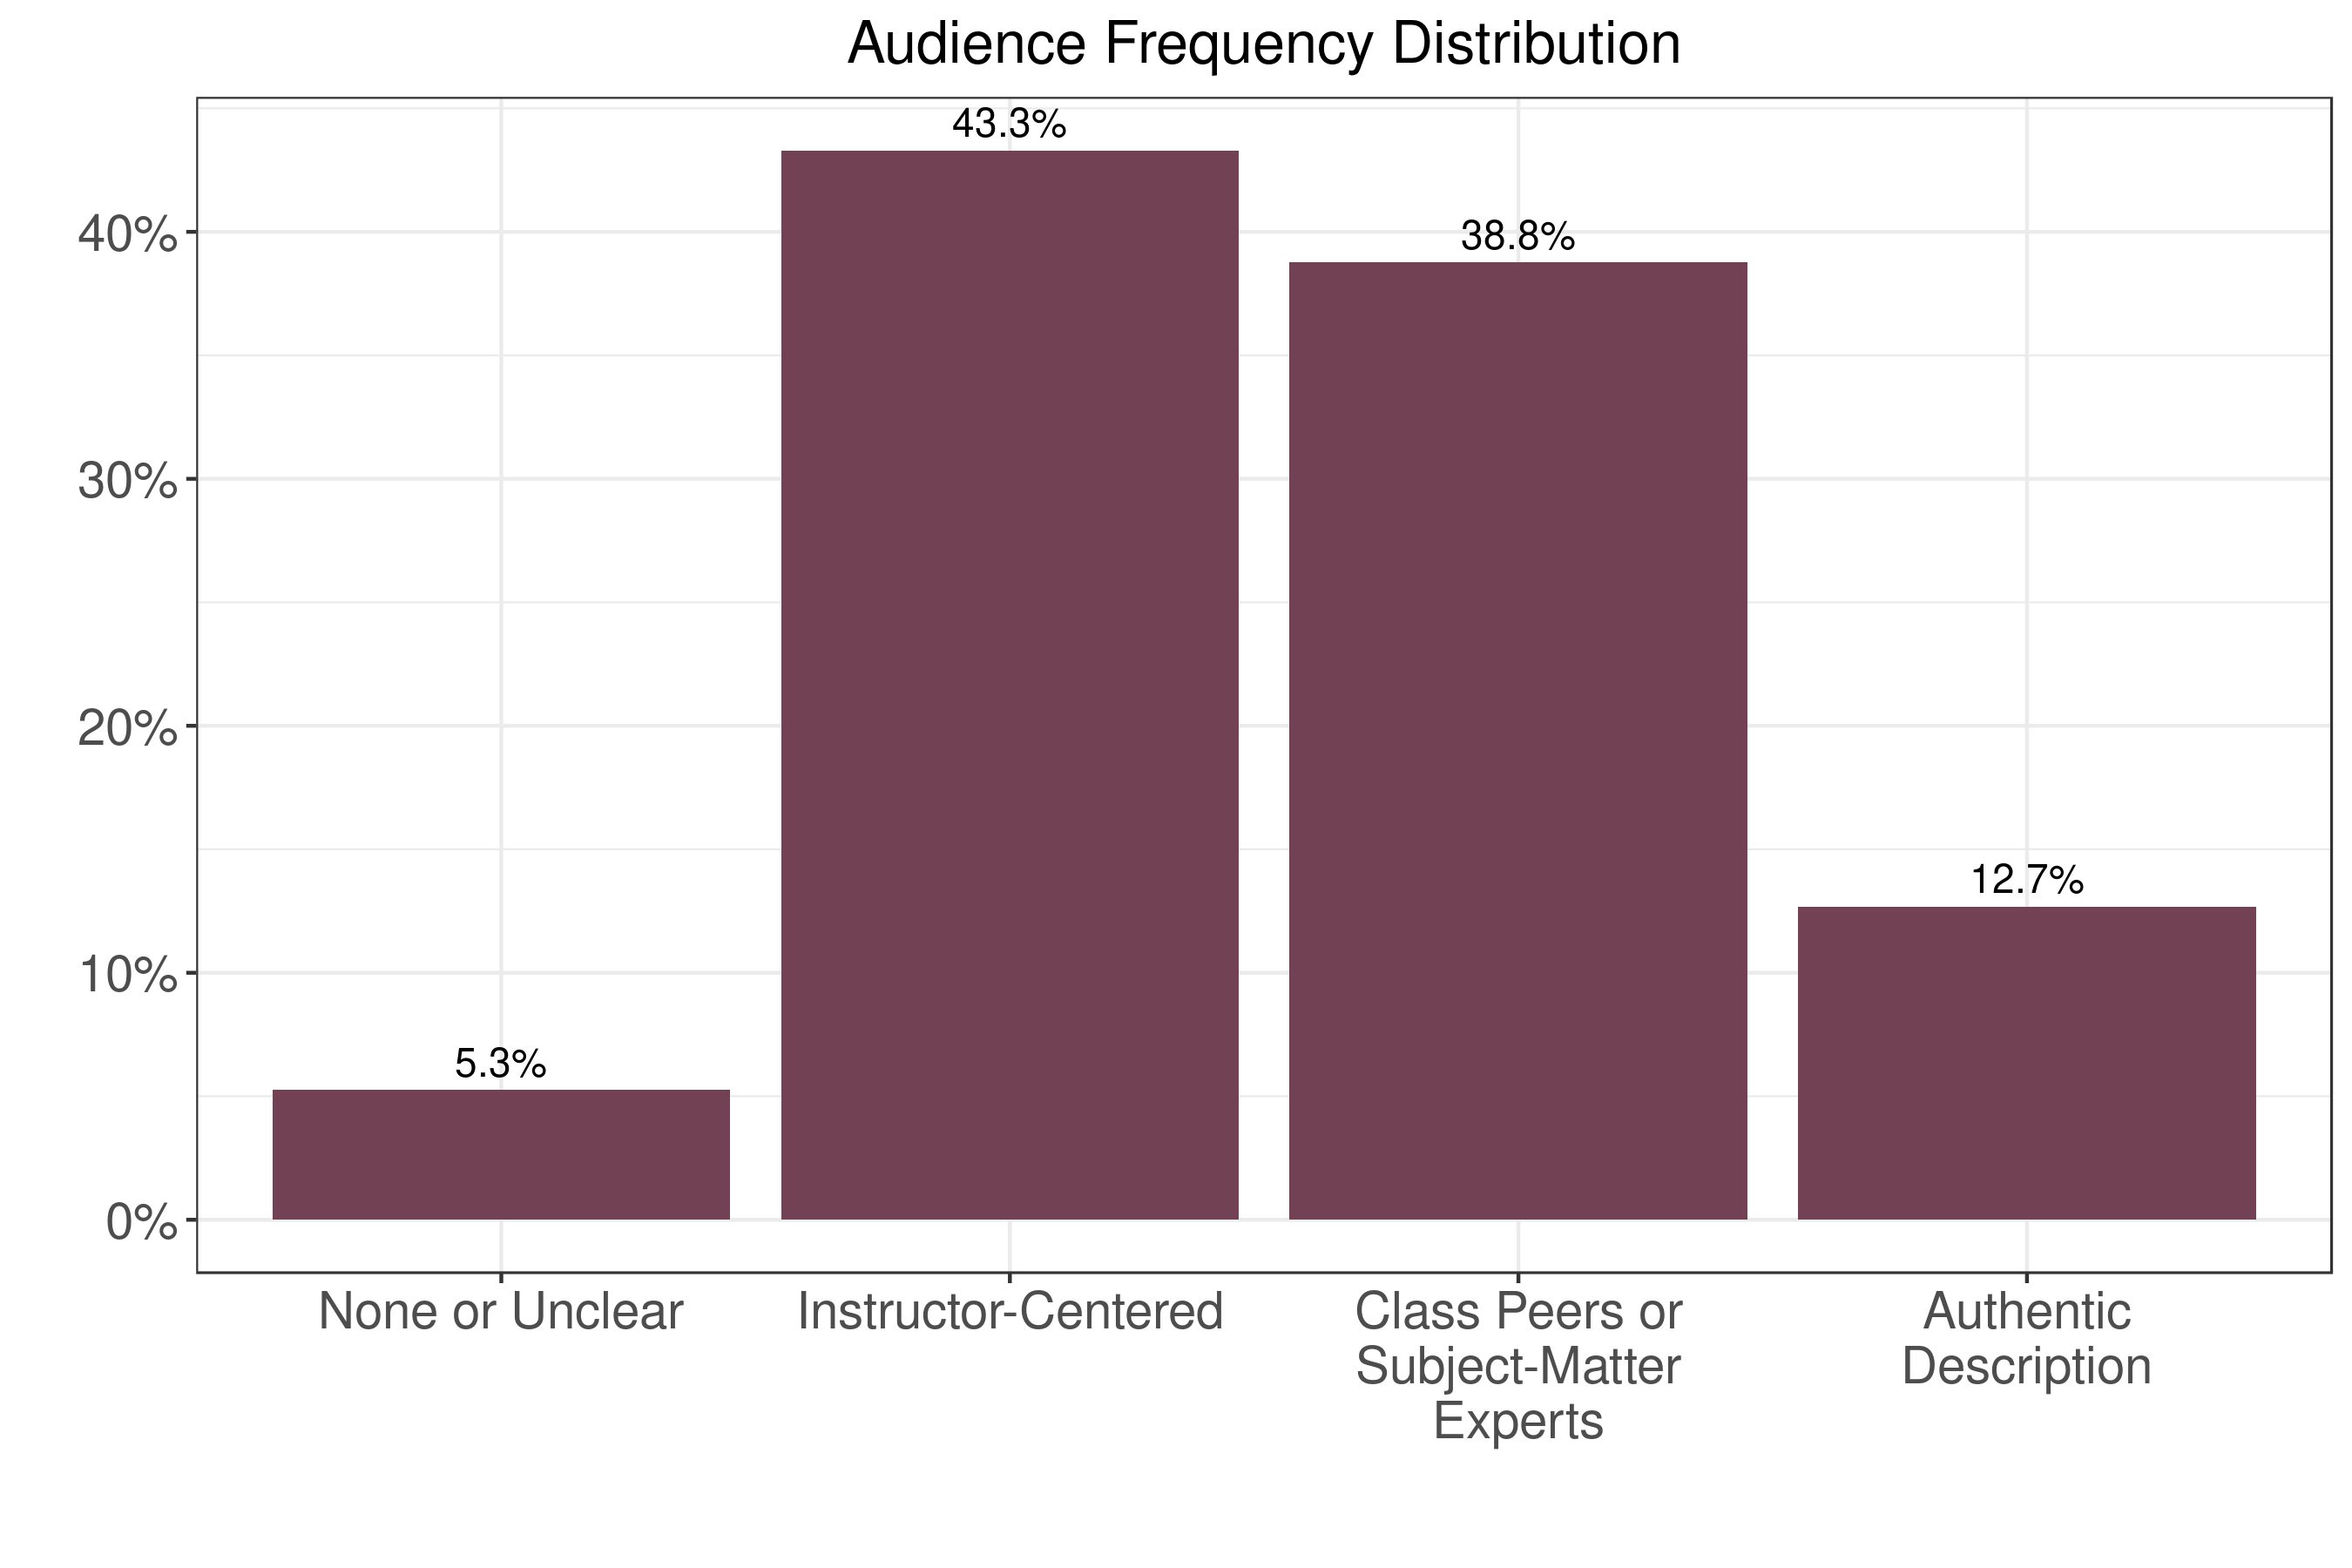
\includegraphics[width=\textwidth]{audience-freq.png}
}

\frame
{
  \ft{Measuring Audience}
  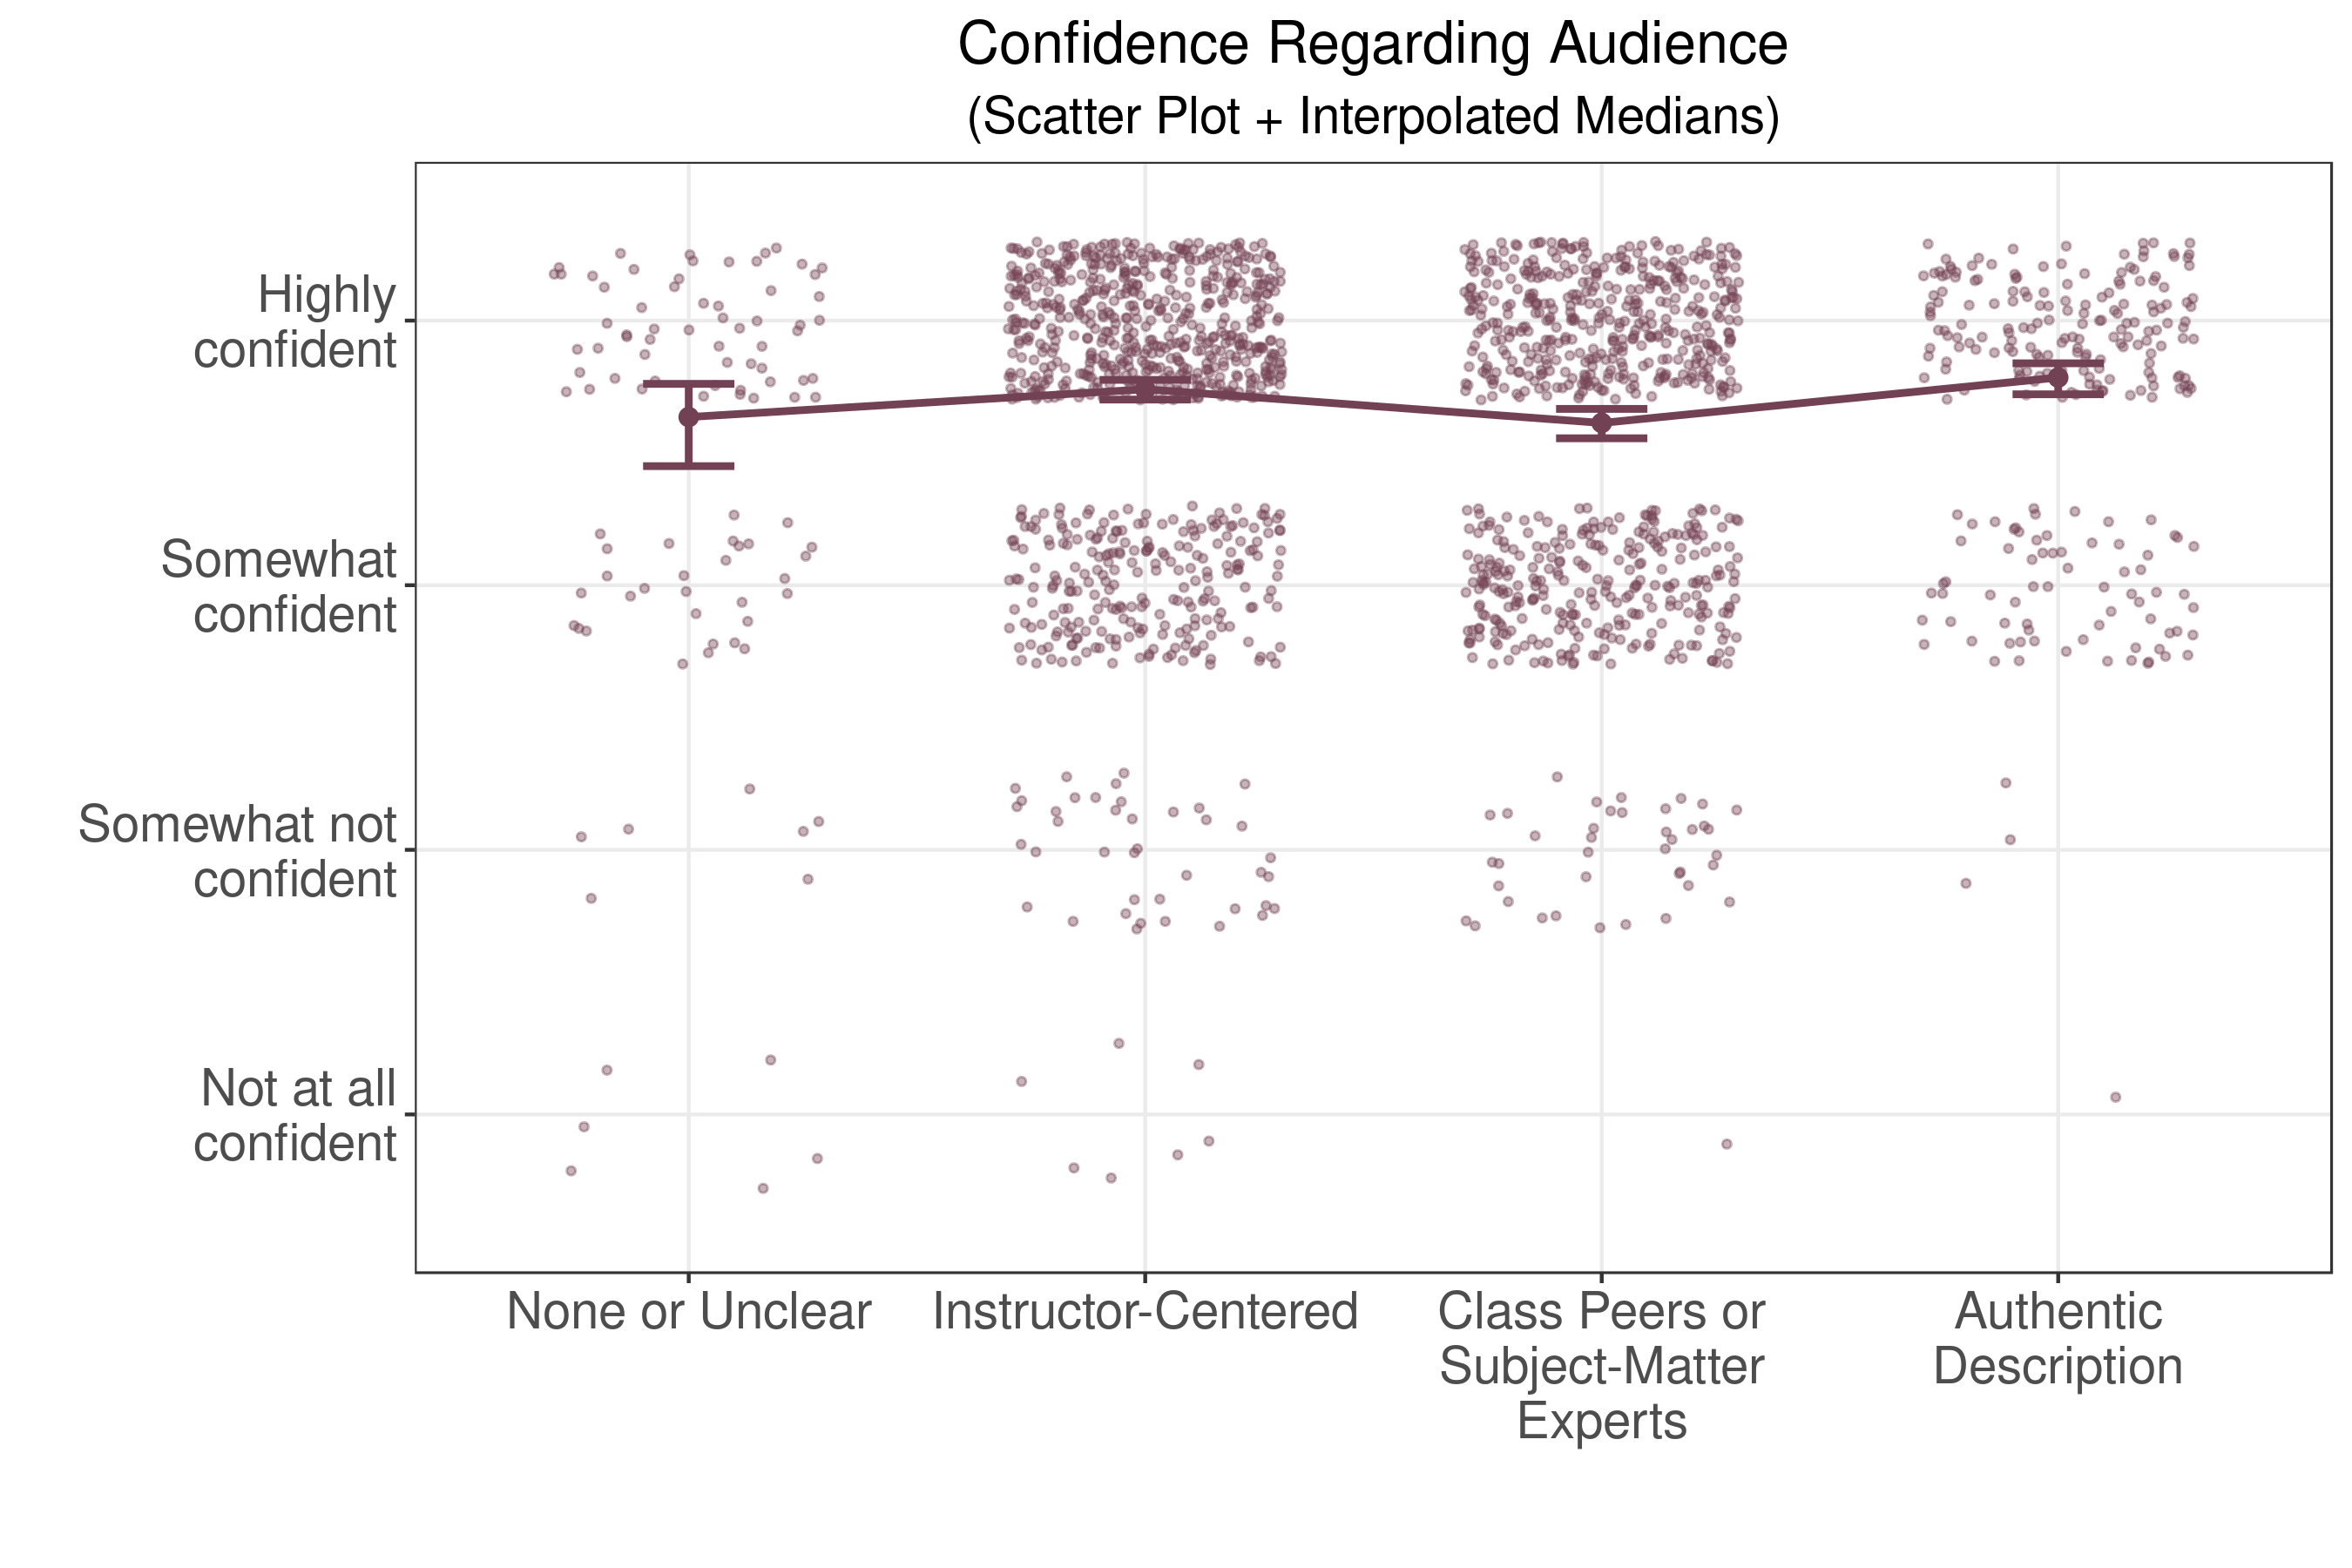
\includegraphics[width=\textwidth]{audience-scat.png}
}

\frame
{
  \ft{Mindset}
  \uncover<+->{
  \begin{block}{What is \textit{Mindset}?}
    An individual's beliefs on learning and intelligence.
  \end{block}}

  \uncover<+->{
  \begin{block}{Fixed Mindset}
    \bi
    \item Abilities come naturally to some, not to others
    \item Prevalent in both low performing and high performing students
    \item \textit{Simply not true.}
    \item \textit{Sets people up for failure.}
      \ei
  \end{block}}

  \uncover<+->{
    \begin{block}{Growth Mindset}
      \bi
      \item Intelligence and ability are not predetermined
      \item Growth in intelligence and ability take work and dedication
      \item \textit{Conducive to learning and success.}
        \ei
  \end{block}
  }
  
}

\frame
{
  \ft{Measuring Mindset}
  Based on Carolyn Dweck (2006)\\
  \textcolor{red}{\url{https://mindsetonline.com/testyourmindset}}

  \begin{center}
    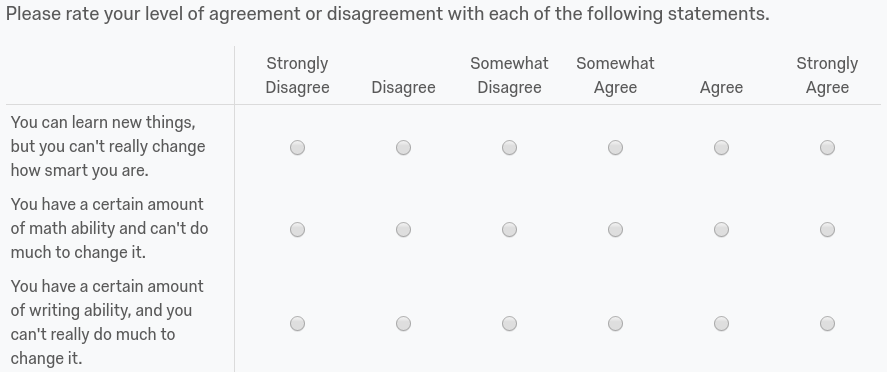
\includegraphics[width=\textwidth]{mindset.png}
  \end{center}
}

\frame
{
  \ft{Mindset Measures}
   \begin{center}
      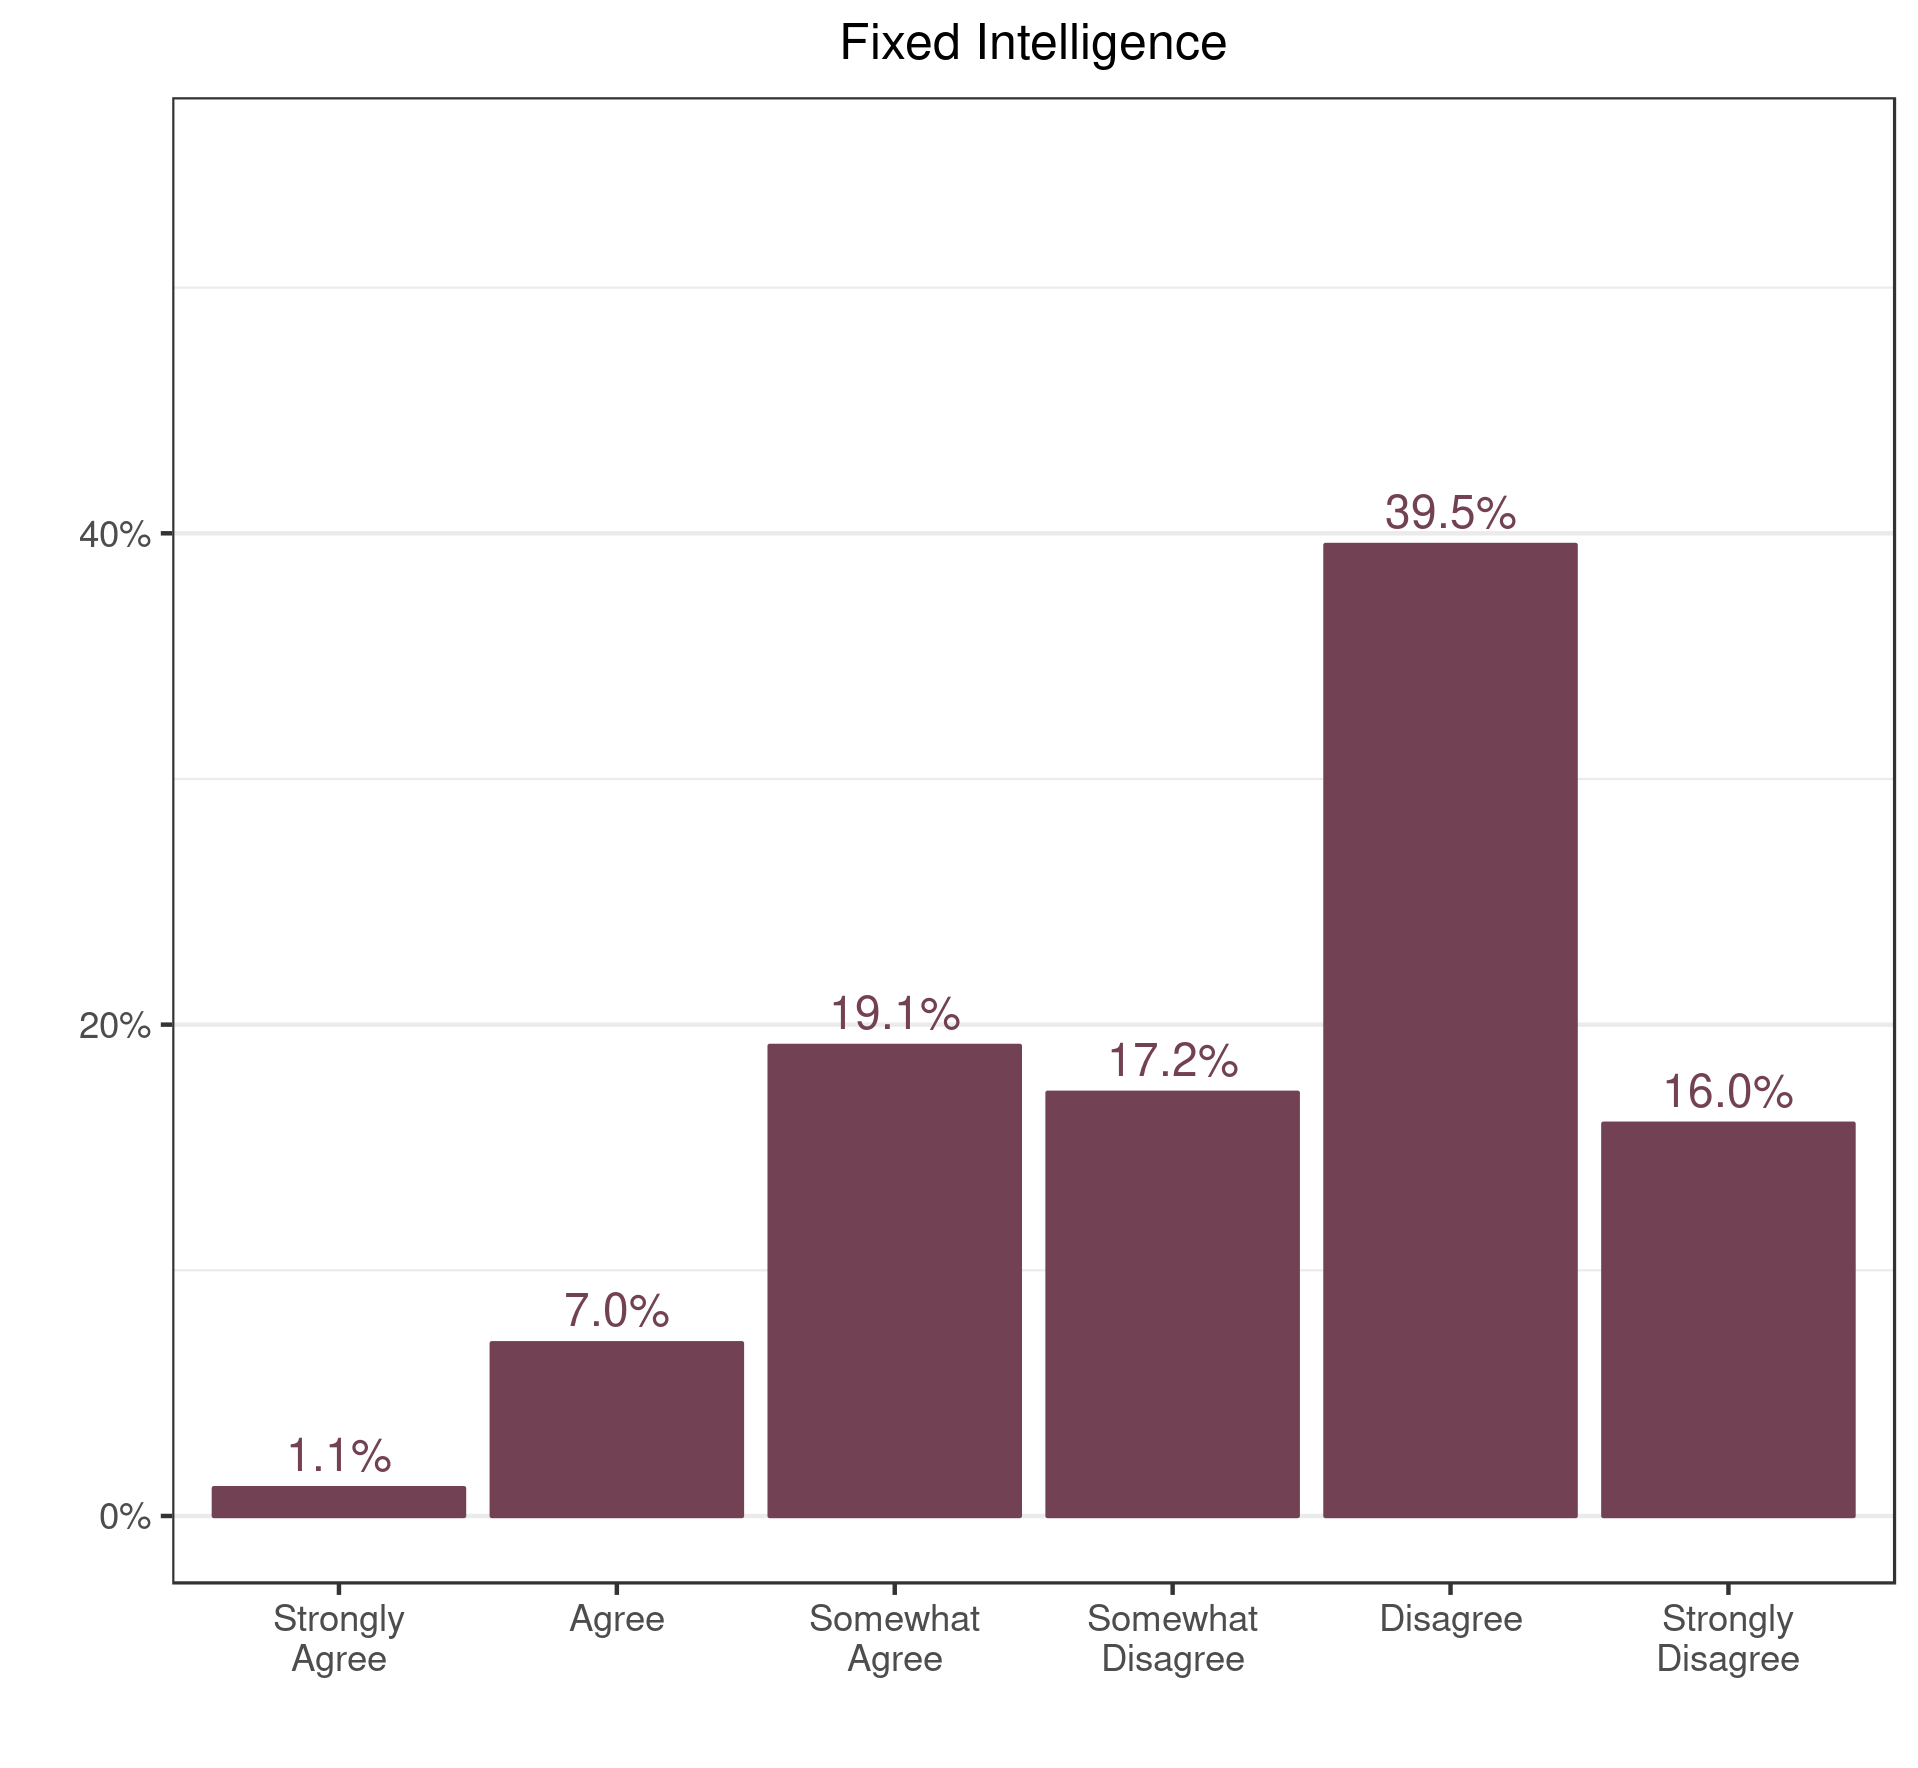
\includegraphics[height=0.9\textheight]{mindhist-smart.png}
   \end{center}    
}

\frame
{
  \ft{Mindset Measures}
   \begin{center}
      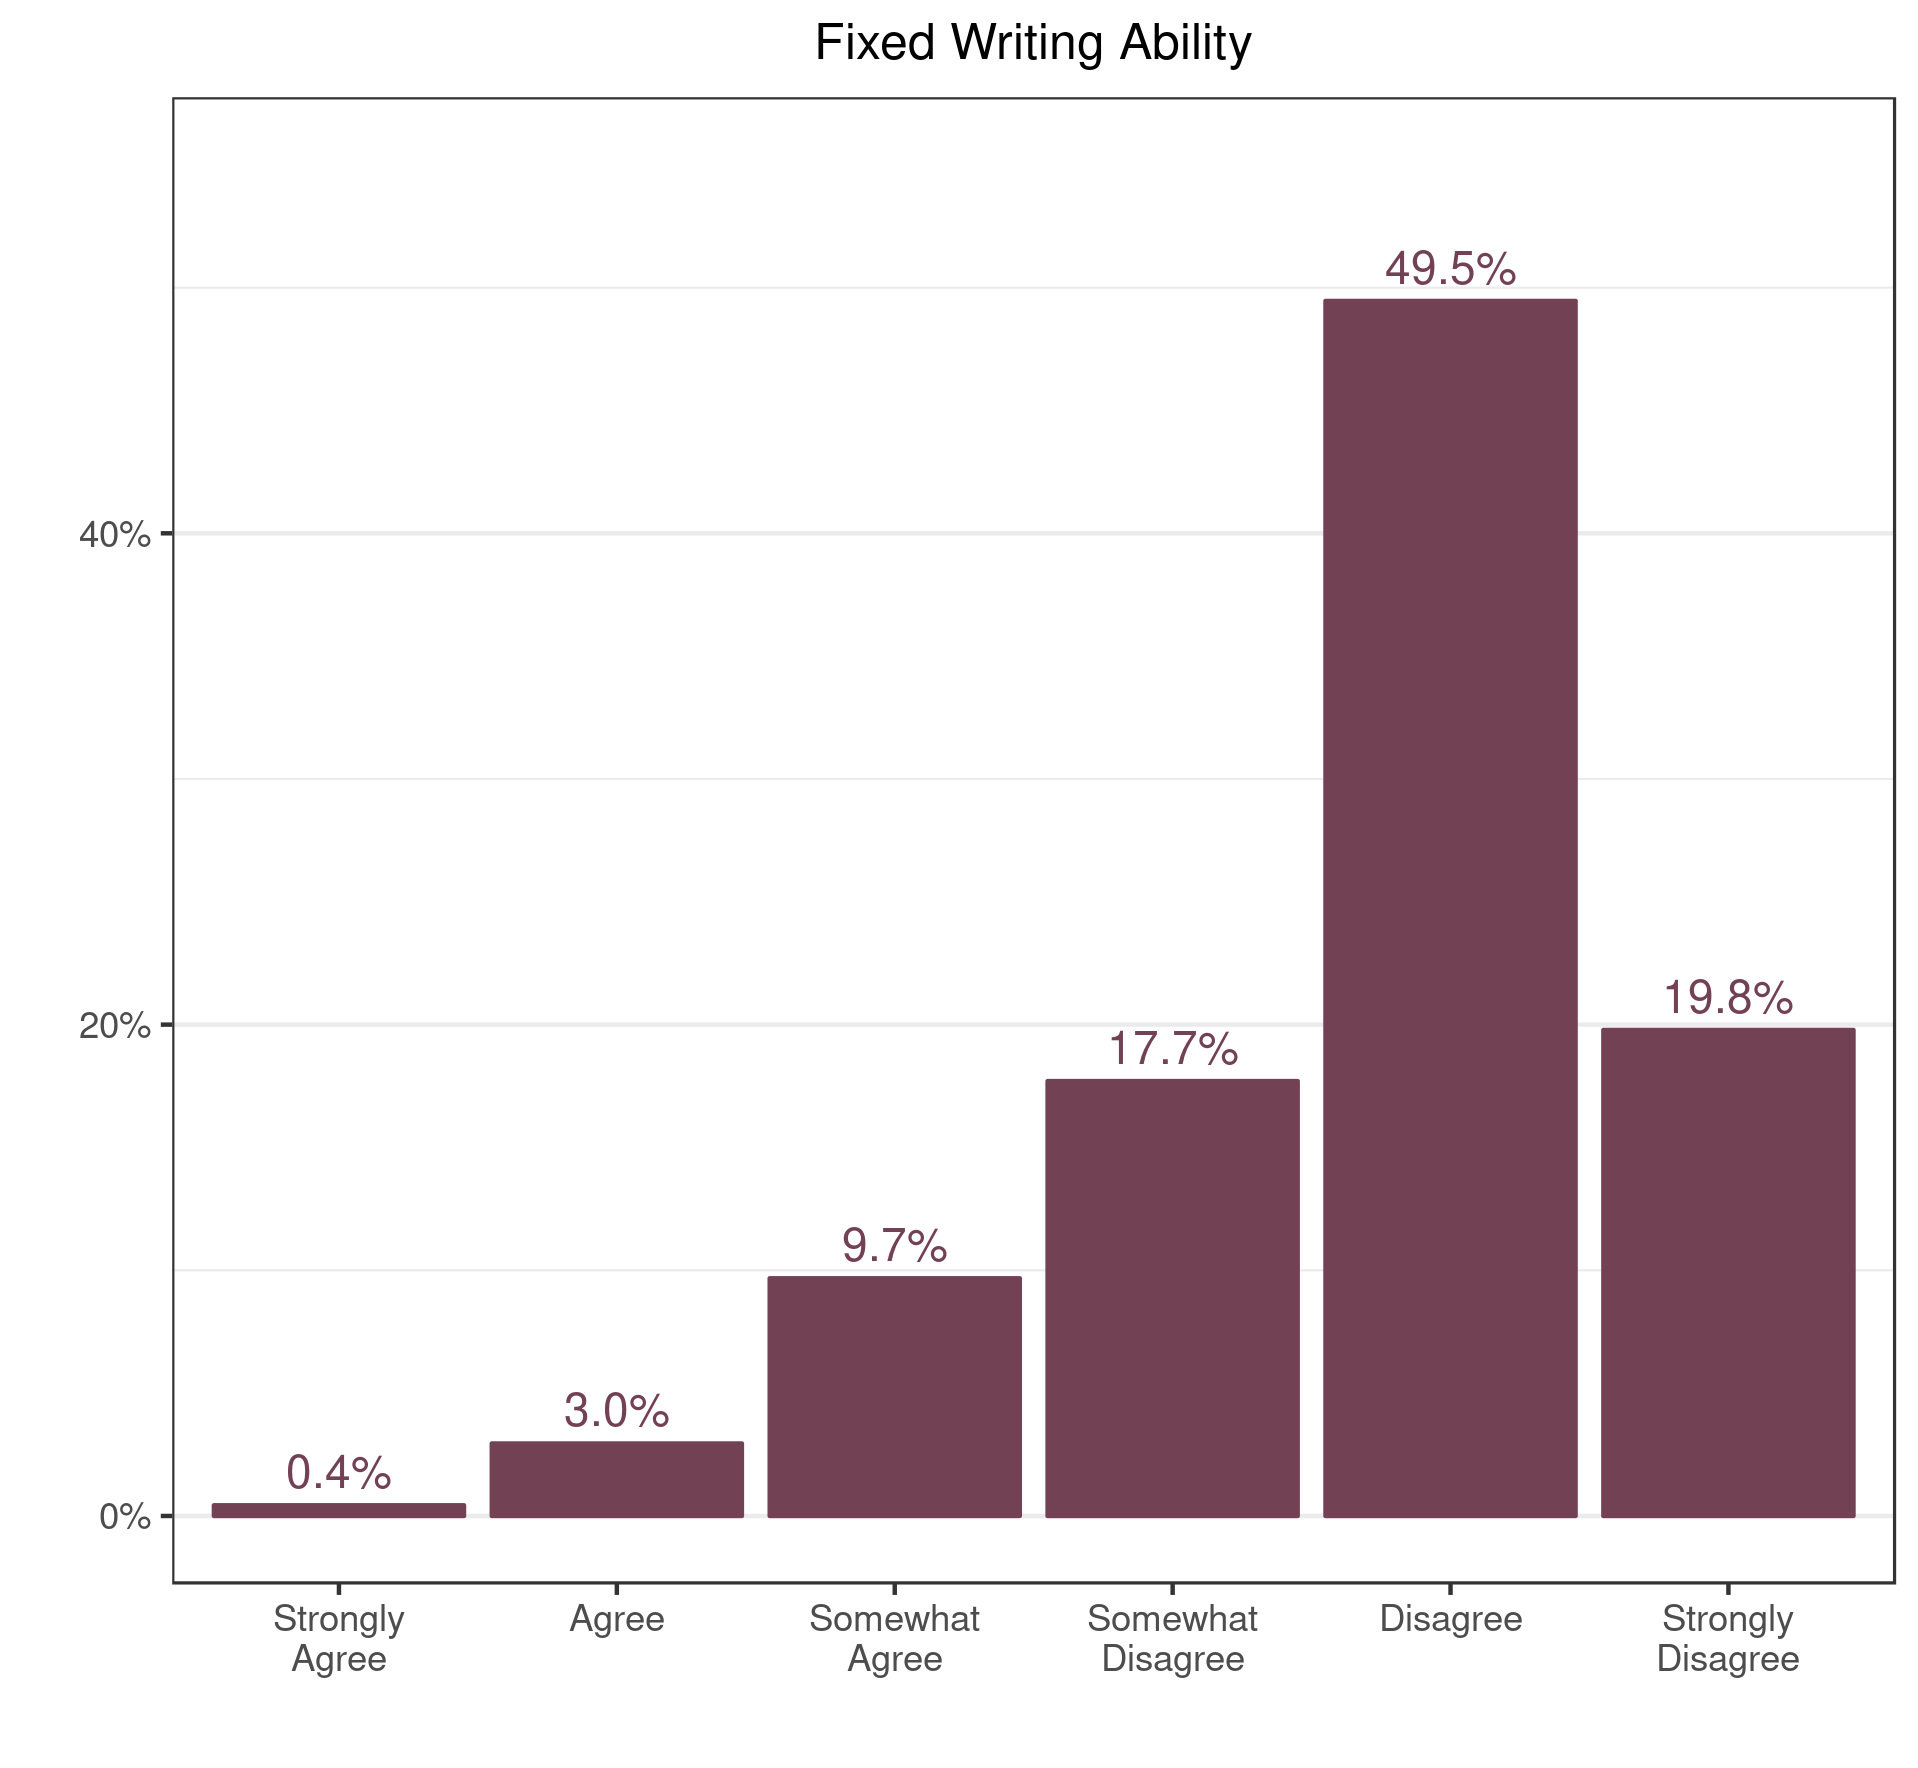
\includegraphics[height=0.9\textheight]{mindhist-math.png}
   \end{center}    
}
\frame
{
  \ft{Mindset Measures}
   \begin{center}
      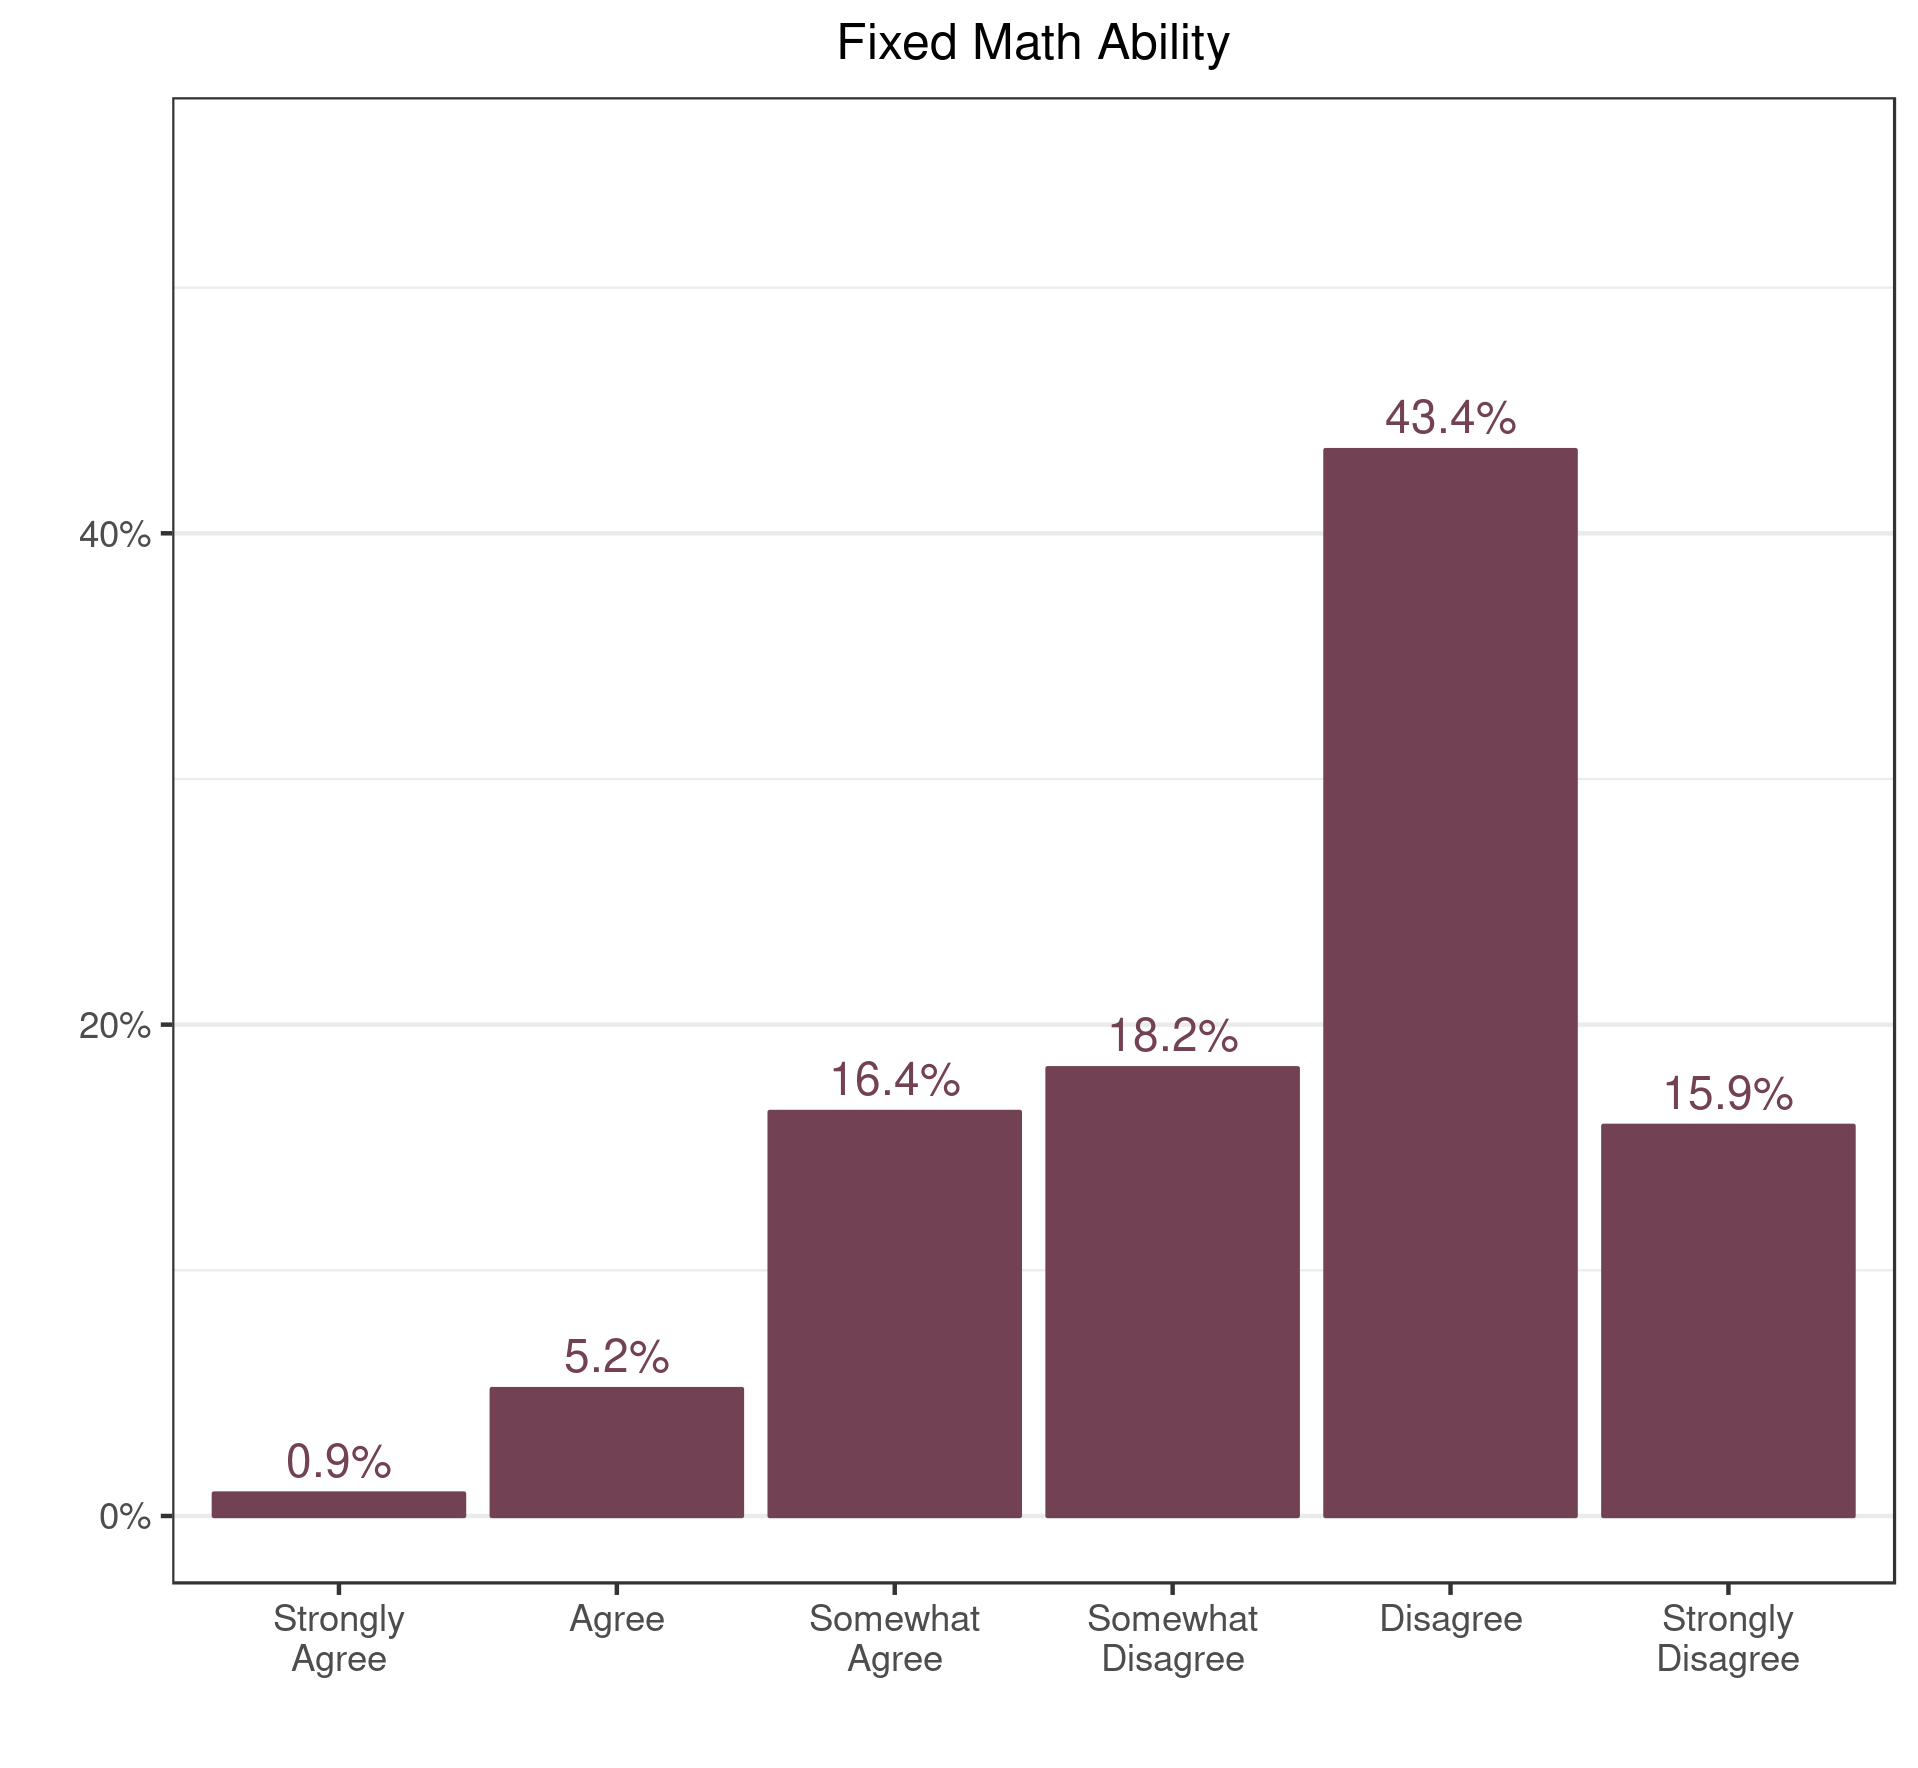
\includegraphics[height=0.9\textheight]{mindhist-write.png}
   \end{center}    
}

\frame
{
  \ft{Mindset Common Factor}
  \bi
  \item Three ordinal measures of mindset
  \item Factor analysis 
  \item Spearman correlation matrix (ranks)
  \ei
} 

\frame
{
  \ft{Mindset Common Factor}
   \begin{center}
      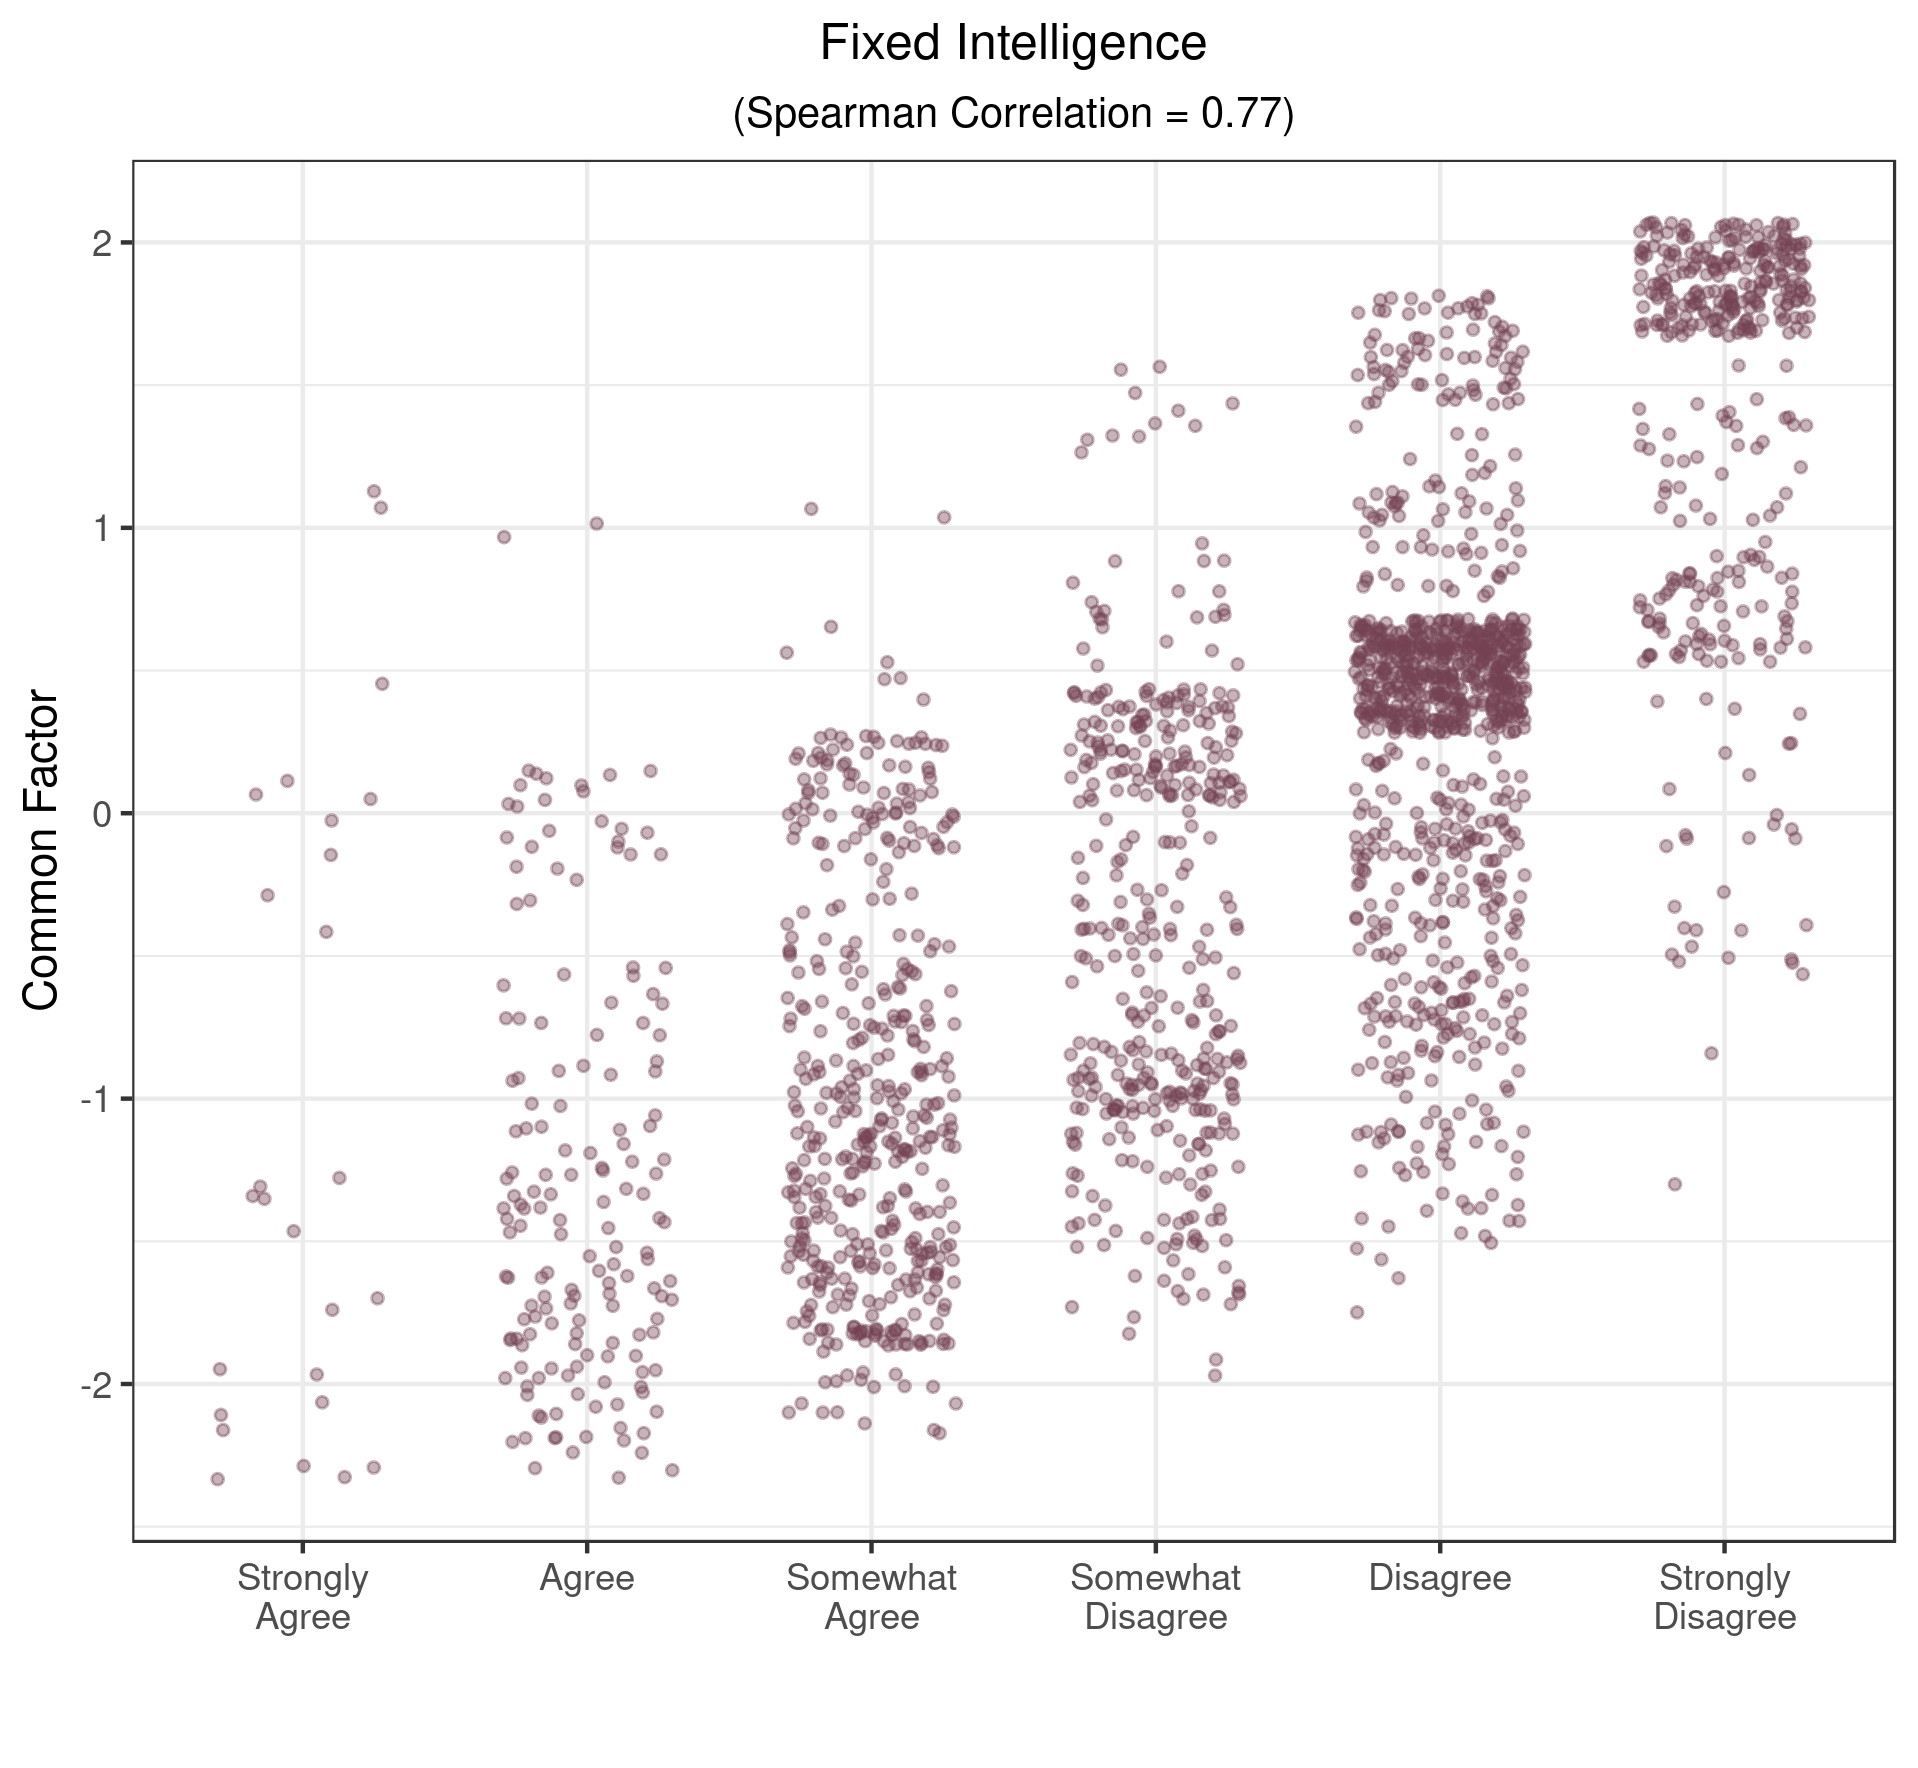
\includegraphics[height=0.9\textheight]{mindscat-smart.png}
   \end{center}    
}

\frame
{
  \ft{Mindset Common Factor}
   \begin{center}
      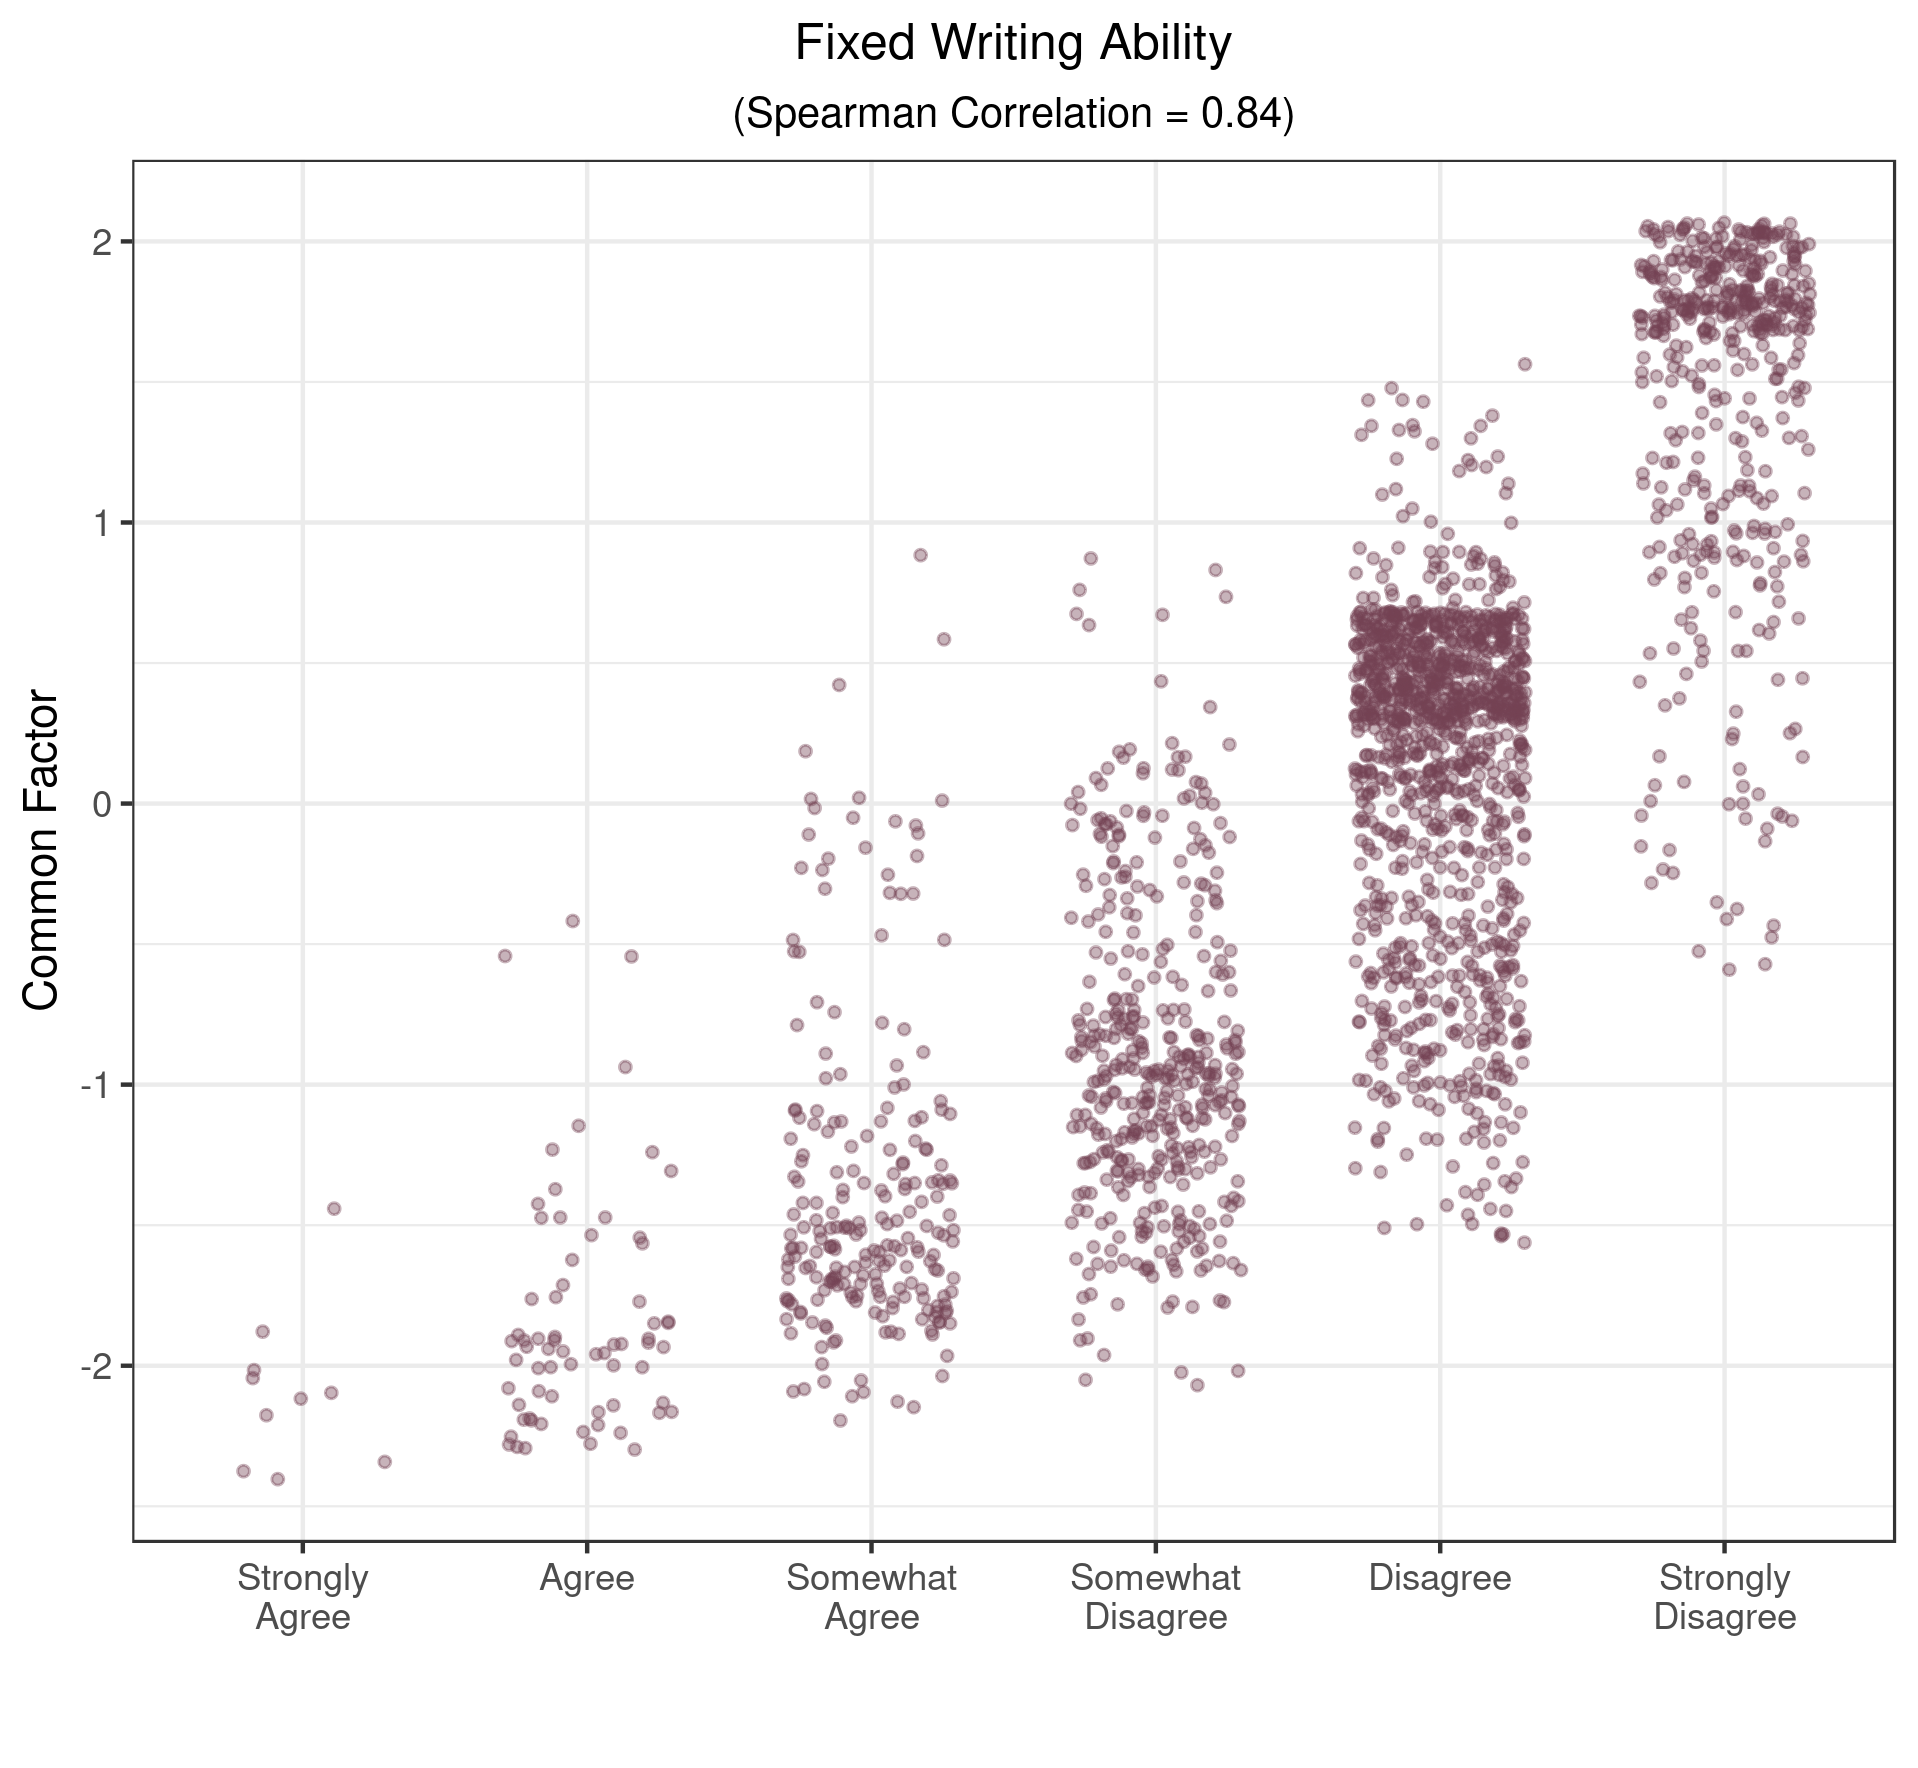
\includegraphics[height=0.9\textheight]{mindscat-math.png}
   \end{center}    
}
\frame
{
  \ft{Mindset Common Factor}
   \begin{center}
      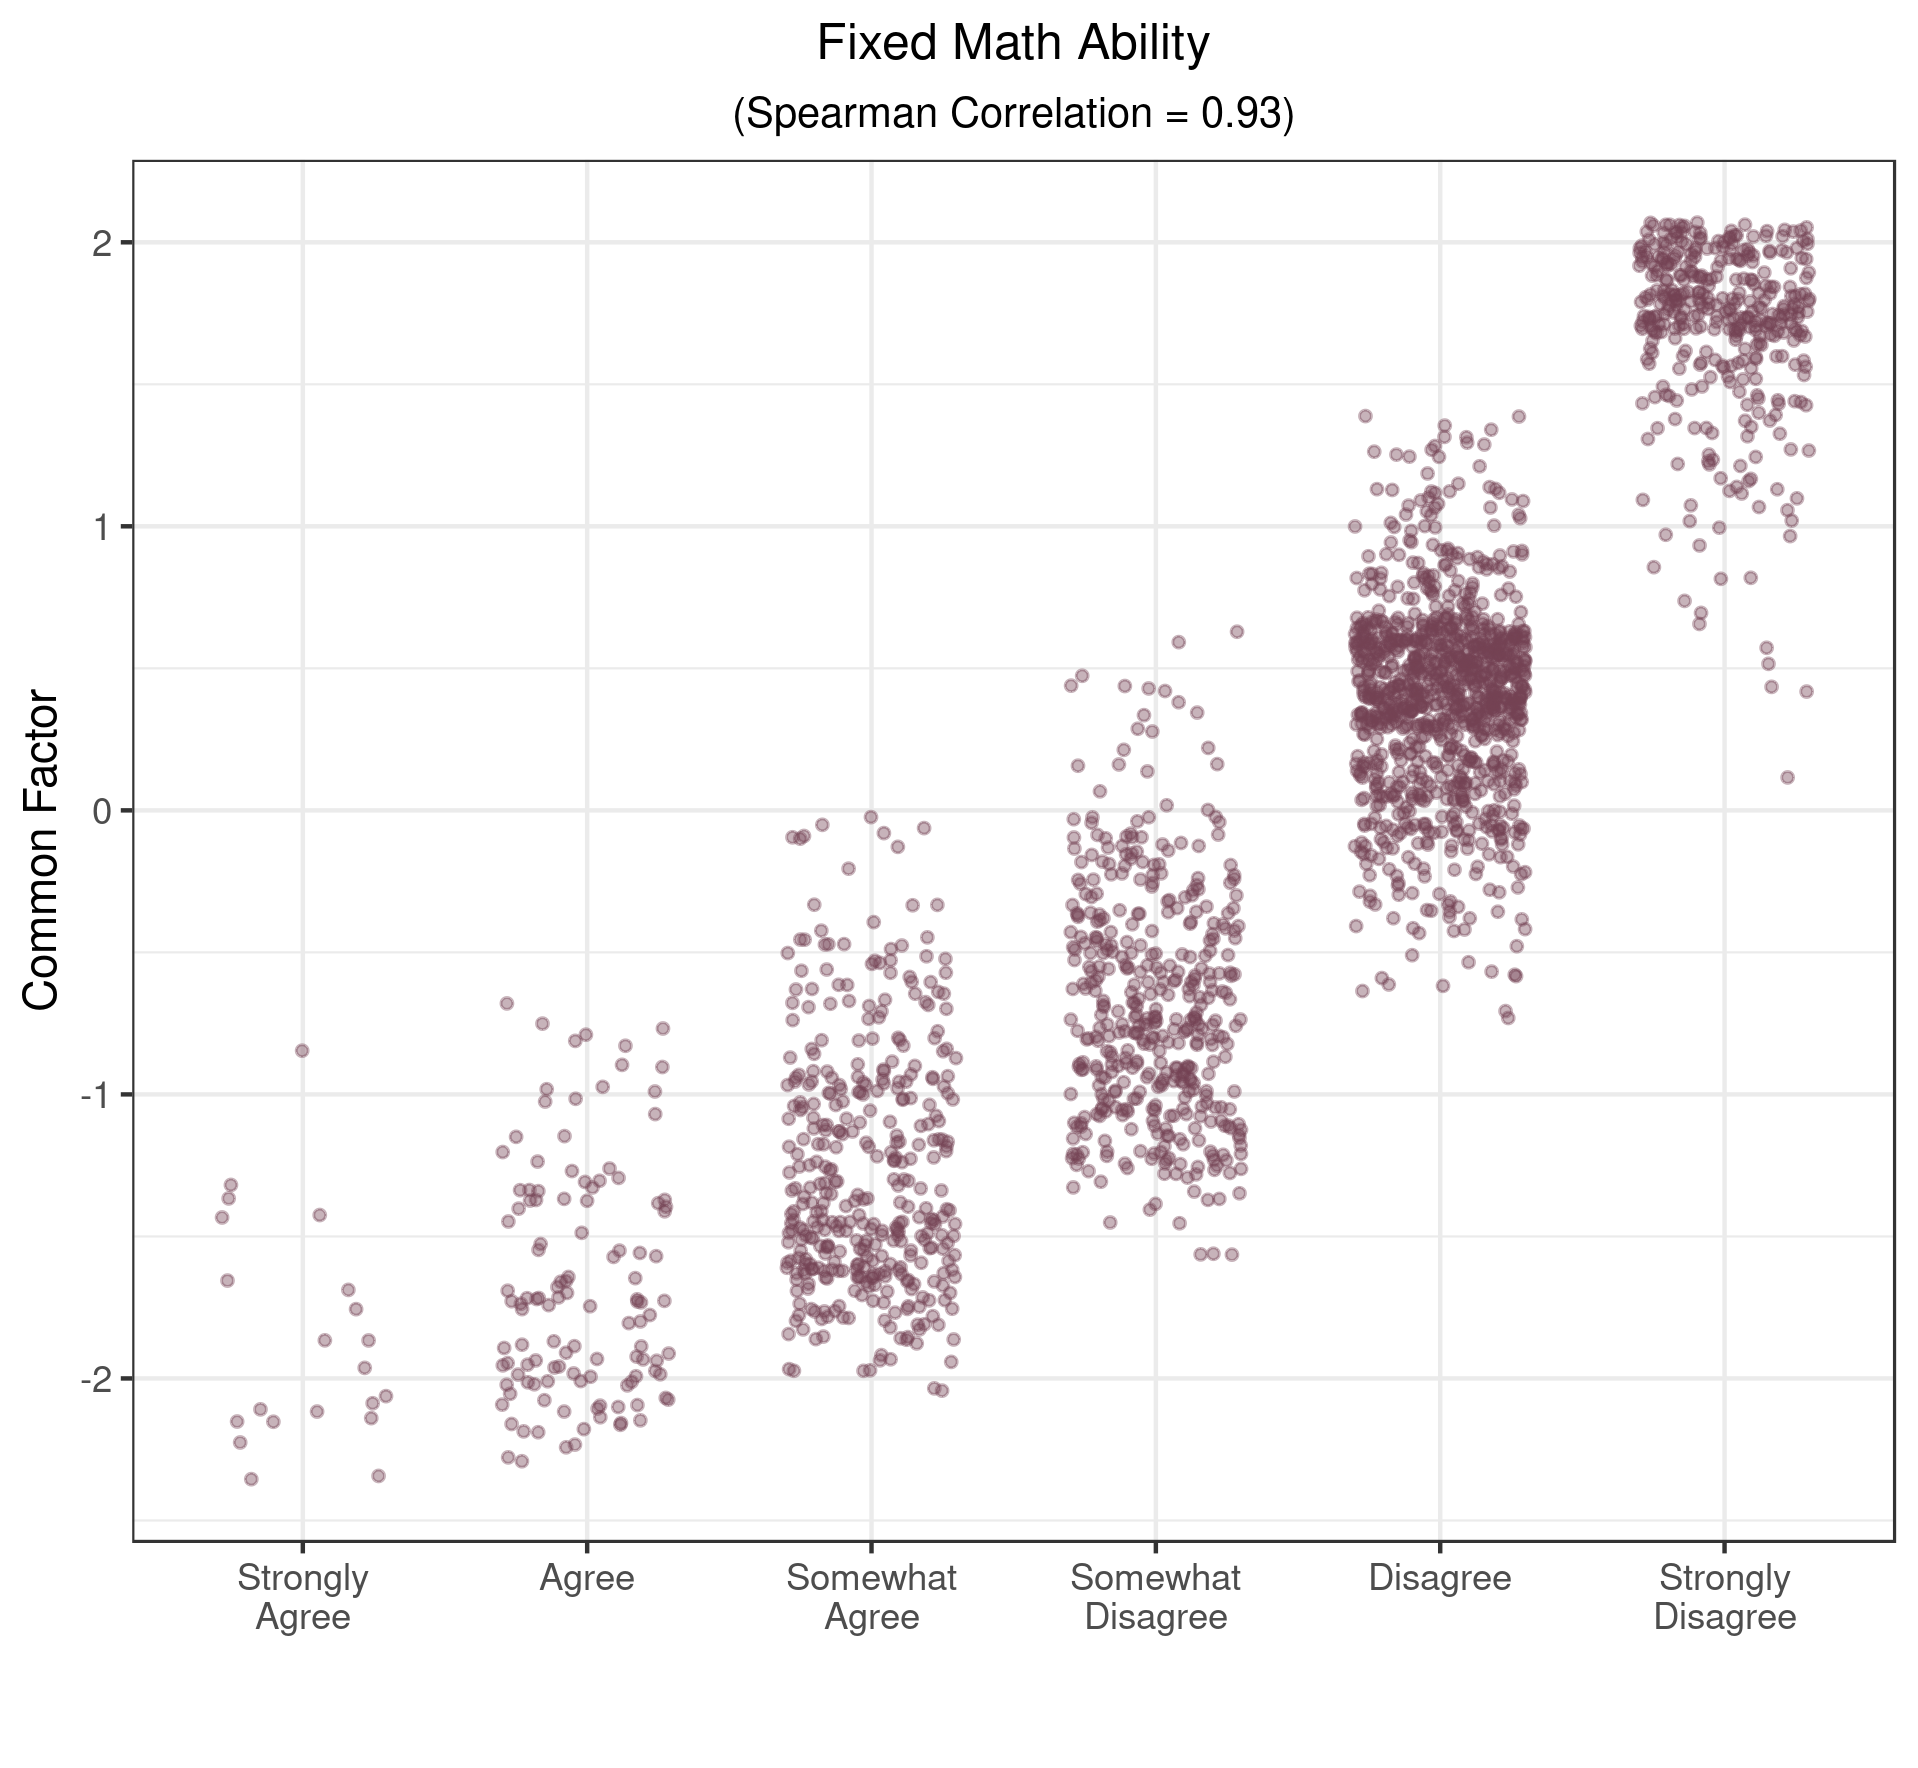
\includegraphics[height=0.9\textheight]{mindscat-write.png}
   \end{center}    
}

\frame
{
  \ft{Explanatory Variables}
  \uncover<+->{
  \begin{block}{Student Mindset}
    \begin{itemize}
    \item \textbf{Fixed:} Belief that intelligence is a fixed trait
    \item \textbf{Growth:} Intelligence is developed with work and dedication
    \end{itemize}
  \end{block}}

  \uncover<+->{
  \begin{block}{Instructor Actions}
    \begin{itemize}
    \item Encourage students to use writing center
    \item Give feedback prior to final draft
    \end{itemize}
  \end{block}}

  \uncover<+->{
  \begin{block}{Student Demographics / Background}
    \begin{columns}[t]
      \column{0.2\textwidth}
      \vspace*{-0.7pc}\begin{itemize}
      \item Gender
      \item Race
      \end{itemize}

      \column{0.7\textwidth}
      \vspace*{-0.7pc}\begin{itemize}
      \item Parents' Education
      \item High school performance: ACT Score
      \end{itemize}
    \end{columns}
  \end{block}}


  \uncover<+->{
  \begin{block}{Academic Characteristics}
    \begin{columns}[t]
      \column{0.4\textwidth}
      \vspace*{-0.7pc}\begin{itemize}
      \item Credits accumulated
      \item Field of study
      \end{itemize}
      
      \column{0.55\textwidth}
      \vspace*{-0.7pc}\begin{itemize}
      \item University identifier
      \end{itemize}
      \end{columns}
  \end{block}}
}

\frame
{
  \ft{Explaining \textbf{Purpose}: Ordered Logit Results}
  \scriptsize{
  \uncover<+->{
  \begin{block}{Mindset and Instructor Influences}
    \begin{tabular}{p{2in}cl}
      \textbf{Variable} & \textbf{Coefficient} & \textbf{P-value} \\ \hline
       Mindset Common Factor & 		 0.093 	&	 0.039**\\
       Instructor Feedback & 		 0.345 	& 	 0.001***\\
       Writing Center Encouragement & 		 0.215 	 & 	 0.098*
    \end{tabular}
  \end{block}
  }
  \uncover<+->{
  \begin{block}{Demographics}
    \begin{tabular}{p{2in}cl}
      \textbf{Variable} & \textbf{Coefficient} & \textbf{P-value} \\ \hline
      Female &		 0.121 	 & 	 0.279 \\
      Race: Non-white &		 -0.420 	&	 0.030** \\
      Parent w/ no college education &	 -0.160 	& 	 0.302  \\
      ACT Score &	 0.076 	 & 	 0.123 
    \end{tabular}
  \end{block}
  }
  \uncover<+->{
  \begin{block}{Academics}
    \begin{tabular}{p{2in}cl}
      \textbf{Variable} & \textbf{Coefficient} & \textbf{P-value} \\ \hline
      Credits Accumulated & -0.200 	&	 0.000***\\
      Field: Education &	 -0.042 	 & 	 0.824 \\
      Field: Liberal Studies &		 -0.045 	 & 	 0.757 \\
      Field: Science/Health &		 0.130 	 &	 0.314 \\
      Omitted field: Business & & 
    \end{tabular}
  \end{block}
  }
}
}
      

\frame
{
  \ft{Explaining \textbf{Audience}: Ordered Logit Results}
  \scriptsize{
  \uncover<+->{
  \begin{block}{Mindset and Instructor Influences}
    \begin{tabular}{p{2in}cl}
      \textbf{Variable} & \textbf{Coefficient} & \textbf{P-value} \\ \hline
       Mindset Common Factor & 		 0.085 	 & 	 0.044** \\
       Instructor Feedback & 		 0.330 	 & 	 0.001*** \\
       Writing Center Encouragement &    0.274 	 & 	 0.024** \\
    \end{tabular}
  \end{block}
  }
  \uncover<+->{
  \begin{block}{Demographics}
    \begin{tabular}{p{2in}cl}
      \textbf{Variable} & \textbf{Coefficient} & \textbf{P-value} \\ \hline
      Female &	 	          0.061 	 &	 0.556 \\
      Race: Non-white & 	         -0.233 	 & 	 0.210 \\
      Parent w/ no college education &   0.077 	 & 	 0.593 \\
      ACT Score & 		 0.062 	 & 	 0.180 
    \end{tabular}
  \end{block}
  }
  \uncover<+->{
  \begin{block}{Academics}
    \begin{tabular}{p{2in}cl}
      \textbf{Variable} & \textbf{Coefficient} & \textbf{P-value} \\ \hline
      Credits Accumulated & 0.046 & 	 0.317 \\
        Field: Education &		 -0.452 	 &	 0.011** \\
        Field: Liberal Studies 	&	 -0.245 	 &	 0.077* \\
        Field: Science/Health &		 -0.189 	 & 	 0.126 \\
        Omitted field: Business & & 
    \end{tabular}
  \end{block}
  }
}
}

\frame
{
  \ft{Conclusions}
  \uncover<+->{
  \begin{block}{Student Experience}
    \begin{itemize}
    \item Most report \textbf{lower-order} writing experiences for \textbf{both purpose and audience}
    \item Does not progress with progression toward degree
    \item Business and science fields - Higher order for \textit{audience}
    \end{itemize}
  \end{block}
  }

  \uncover<+->{
  \begin{block}{Mindset and Instructor Influences}
    \textbf{We can influence students perceptions / experience}
    \begin{itemize}
    \item Encourage a growth mindset\newline
      Ideas from Stanford researchers:\newline \textcolor{red}{\url{https://www.mindsetkit.org/}}
    \item Give students feedback
    \item Send students to the writing center
    \end{itemize}
  \end{block}
  }
}

\end{document}

